
% Default to the notebook output style

    


% Inherit from the specified cell style.




    
\documentclass[11pt]{article}

    
    
    \usepackage[T1]{fontenc}
    % Nicer default font (+ math font) than Computer Modern for most use cases
    \usepackage{mathpazo}

    % Basic figure setup, for now with no caption control since it's done
    % automatically by Pandoc (which extracts ![](path) syntax from Markdown).
    \usepackage{graphicx}
    % We will generate all images so they have a width \maxwidth. This means
    % that they will get their normal width if they fit onto the page, but
    % are scaled down if they would overflow the margins.
    \makeatletter
    \def\maxwidth{\ifdim\Gin@nat@width>\linewidth\linewidth
    \else\Gin@nat@width\fi}
    \makeatother
    \let\Oldincludegraphics\includegraphics
    % Set max figure width to be 80% of text width, for now hardcoded.
    \renewcommand{\includegraphics}[1]{\Oldincludegraphics[width=.8\maxwidth]{#1}}
    % Ensure that by default, figures have no caption (until we provide a
    % proper Figure object with a Caption API and a way to capture that
    % in the conversion process - todo).
    \usepackage{caption}
    \DeclareCaptionLabelFormat{nolabel}{}
    \captionsetup{labelformat=nolabel}

    \usepackage{adjustbox} % Used to constrain images to a maximum size 
    \usepackage{xcolor} % Allow colors to be defined
    \usepackage{enumerate} % Needed for markdown enumerations to work
    \usepackage{geometry} % Used to adjust the document margins
    \usepackage{amsmath} % Equations
    \usepackage{amssymb} % Equations
    \usepackage{textcomp} % defines textquotesingle
    % Hack from http://tex.stackexchange.com/a/47451/13684:
    \AtBeginDocument{%
        \def\PYZsq{\textquotesingle}% Upright quotes in Pygmentized code
    }
    \usepackage{upquote} % Upright quotes for verbatim code
    \usepackage{eurosym} % defines \euro
    \usepackage[mathletters]{ucs} % Extended unicode (utf-8) support
    \usepackage[utf8x]{inputenc} % Allow utf-8 characters in the tex document
    \usepackage{fancyvrb} % verbatim replacement that allows latex
    \usepackage{grffile} % extends the file name processing of package graphics 
                         % to support a larger range 
    % The hyperref package gives us a pdf with properly built
    % internal navigation ('pdf bookmarks' for the table of contents,
    % internal cross-reference links, web links for URLs, etc.)
    \usepackage{hyperref}
    \usepackage{longtable} % longtable support required by pandoc >1.10
    \usepackage{booktabs}  % table support for pandoc > 1.12.2
    \usepackage[inline]{enumitem} % IRkernel/repr support (it uses the enumerate* environment)
    \usepackage[normalem]{ulem} % ulem is needed to support strikethroughs (\sout)
                                % normalem makes italics be italics, not underlines
    

    
    
    % Colors for the hyperref package
    \definecolor{urlcolor}{rgb}{0,.145,.698}
    \definecolor{linkcolor}{rgb}{.71,0.21,0.01}
    \definecolor{citecolor}{rgb}{.12,.54,.11}

    % ANSI colors
    \definecolor{ansi-black}{HTML}{3E424D}
    \definecolor{ansi-black-intense}{HTML}{282C36}
    \definecolor{ansi-red}{HTML}{E75C58}
    \definecolor{ansi-red-intense}{HTML}{B22B31}
    \definecolor{ansi-green}{HTML}{00A250}
    \definecolor{ansi-green-intense}{HTML}{007427}
    \definecolor{ansi-yellow}{HTML}{DDB62B}
    \definecolor{ansi-yellow-intense}{HTML}{B27D12}
    \definecolor{ansi-blue}{HTML}{208FFB}
    \definecolor{ansi-blue-intense}{HTML}{0065CA}
    \definecolor{ansi-magenta}{HTML}{D160C4}
    \definecolor{ansi-magenta-intense}{HTML}{A03196}
    \definecolor{ansi-cyan}{HTML}{60C6C8}
    \definecolor{ansi-cyan-intense}{HTML}{258F8F}
    \definecolor{ansi-white}{HTML}{C5C1B4}
    \definecolor{ansi-white-intense}{HTML}{A1A6B2}

    % commands and environments needed by pandoc snippets
    % extracted from the output of `pandoc -s`
    \providecommand{\tightlist}{%
      \setlength{\itemsep}{0pt}\setlength{\parskip}{0pt}}
    \DefineVerbatimEnvironment{Highlighting}{Verbatim}{commandchars=\\\{\}}
    % Add ',fontsize=\small' for more characters per line
    \newenvironment{Shaded}{}{}
    \newcommand{\KeywordTok}[1]{\textcolor[rgb]{0.00,0.44,0.13}{\textbf{{#1}}}}
    \newcommand{\DataTypeTok}[1]{\textcolor[rgb]{0.56,0.13,0.00}{{#1}}}
    \newcommand{\DecValTok}[1]{\textcolor[rgb]{0.25,0.63,0.44}{{#1}}}
    \newcommand{\BaseNTok}[1]{\textcolor[rgb]{0.25,0.63,0.44}{{#1}}}
    \newcommand{\FloatTok}[1]{\textcolor[rgb]{0.25,0.63,0.44}{{#1}}}
    \newcommand{\CharTok}[1]{\textcolor[rgb]{0.25,0.44,0.63}{{#1}}}
    \newcommand{\StringTok}[1]{\textcolor[rgb]{0.25,0.44,0.63}{{#1}}}
    \newcommand{\CommentTok}[1]{\textcolor[rgb]{0.38,0.63,0.69}{\textit{{#1}}}}
    \newcommand{\OtherTok}[1]{\textcolor[rgb]{0.00,0.44,0.13}{{#1}}}
    \newcommand{\AlertTok}[1]{\textcolor[rgb]{1.00,0.00,0.00}{\textbf{{#1}}}}
    \newcommand{\FunctionTok}[1]{\textcolor[rgb]{0.02,0.16,0.49}{{#1}}}
    \newcommand{\RegionMarkerTok}[1]{{#1}}
    \newcommand{\ErrorTok}[1]{\textcolor[rgb]{1.00,0.00,0.00}{\textbf{{#1}}}}
    \newcommand{\NormalTok}[1]{{#1}}
    
    % Additional commands for more recent versions of Pandoc
    \newcommand{\ConstantTok}[1]{\textcolor[rgb]{0.53,0.00,0.00}{{#1}}}
    \newcommand{\SpecialCharTok}[1]{\textcolor[rgb]{0.25,0.44,0.63}{{#1}}}
    \newcommand{\VerbatimStringTok}[1]{\textcolor[rgb]{0.25,0.44,0.63}{{#1}}}
    \newcommand{\SpecialStringTok}[1]{\textcolor[rgb]{0.73,0.40,0.53}{{#1}}}
    \newcommand{\ImportTok}[1]{{#1}}
    \newcommand{\DocumentationTok}[1]{\textcolor[rgb]{0.73,0.13,0.13}{\textit{{#1}}}}
    \newcommand{\AnnotationTok}[1]{\textcolor[rgb]{0.38,0.63,0.69}{\textbf{\textit{{#1}}}}}
    \newcommand{\CommentVarTok}[1]{\textcolor[rgb]{0.38,0.63,0.69}{\textbf{\textit{{#1}}}}}
    \newcommand{\VariableTok}[1]{\textcolor[rgb]{0.10,0.09,0.49}{{#1}}}
    \newcommand{\ControlFlowTok}[1]{\textcolor[rgb]{0.00,0.44,0.13}{\textbf{{#1}}}}
    \newcommand{\OperatorTok}[1]{\textcolor[rgb]{0.40,0.40,0.40}{{#1}}}
    \newcommand{\BuiltInTok}[1]{{#1}}
    \newcommand{\ExtensionTok}[1]{{#1}}
    \newcommand{\PreprocessorTok}[1]{\textcolor[rgb]{0.74,0.48,0.00}{{#1}}}
    \newcommand{\AttributeTok}[1]{\textcolor[rgb]{0.49,0.56,0.16}{{#1}}}
    \newcommand{\InformationTok}[1]{\textcolor[rgb]{0.38,0.63,0.69}{\textbf{\textit{{#1}}}}}
    \newcommand{\WarningTok}[1]{\textcolor[rgb]{0.38,0.63,0.69}{\textbf{\textit{{#1}}}}}
    
    
    % Define a nice break command that doesn't care if a line doesn't already
    % exist.
    \def\br{\hspace*{\fill} \\* }
    % Math Jax compatability definitions
    \def\gt{>}
    \def\lt{<}
    % Document parameters
    \title{1 - Sequence to Sequence Learning with Neural Networks}
    
    
    

    % Pygments definitions
    
\makeatletter
\def\PY@reset{\let\PY@it=\relax \let\PY@bf=\relax%
    \let\PY@ul=\relax \let\PY@tc=\relax%
    \let\PY@bc=\relax \let\PY@ff=\relax}
\def\PY@tok#1{\csname PY@tok@#1\endcsname}
\def\PY@toks#1+{\ifx\relax#1\empty\else%
    \PY@tok{#1}\expandafter\PY@toks\fi}
\def\PY@do#1{\PY@bc{\PY@tc{\PY@ul{%
    \PY@it{\PY@bf{\PY@ff{#1}}}}}}}
\def\PY#1#2{\PY@reset\PY@toks#1+\relax+\PY@do{#2}}

\expandafter\def\csname PY@tok@w\endcsname{\def\PY@tc##1{\textcolor[rgb]{0.73,0.73,0.73}{##1}}}
\expandafter\def\csname PY@tok@c\endcsname{\let\PY@it=\textit\def\PY@tc##1{\textcolor[rgb]{0.25,0.50,0.50}{##1}}}
\expandafter\def\csname PY@tok@cp\endcsname{\def\PY@tc##1{\textcolor[rgb]{0.74,0.48,0.00}{##1}}}
\expandafter\def\csname PY@tok@k\endcsname{\let\PY@bf=\textbf\def\PY@tc##1{\textcolor[rgb]{0.00,0.50,0.00}{##1}}}
\expandafter\def\csname PY@tok@kp\endcsname{\def\PY@tc##1{\textcolor[rgb]{0.00,0.50,0.00}{##1}}}
\expandafter\def\csname PY@tok@kt\endcsname{\def\PY@tc##1{\textcolor[rgb]{0.69,0.00,0.25}{##1}}}
\expandafter\def\csname PY@tok@o\endcsname{\def\PY@tc##1{\textcolor[rgb]{0.40,0.40,0.40}{##1}}}
\expandafter\def\csname PY@tok@ow\endcsname{\let\PY@bf=\textbf\def\PY@tc##1{\textcolor[rgb]{0.67,0.13,1.00}{##1}}}
\expandafter\def\csname PY@tok@nb\endcsname{\def\PY@tc##1{\textcolor[rgb]{0.00,0.50,0.00}{##1}}}
\expandafter\def\csname PY@tok@nf\endcsname{\def\PY@tc##1{\textcolor[rgb]{0.00,0.00,1.00}{##1}}}
\expandafter\def\csname PY@tok@nc\endcsname{\let\PY@bf=\textbf\def\PY@tc##1{\textcolor[rgb]{0.00,0.00,1.00}{##1}}}
\expandafter\def\csname PY@tok@nn\endcsname{\let\PY@bf=\textbf\def\PY@tc##1{\textcolor[rgb]{0.00,0.00,1.00}{##1}}}
\expandafter\def\csname PY@tok@ne\endcsname{\let\PY@bf=\textbf\def\PY@tc##1{\textcolor[rgb]{0.82,0.25,0.23}{##1}}}
\expandafter\def\csname PY@tok@nv\endcsname{\def\PY@tc##1{\textcolor[rgb]{0.10,0.09,0.49}{##1}}}
\expandafter\def\csname PY@tok@no\endcsname{\def\PY@tc##1{\textcolor[rgb]{0.53,0.00,0.00}{##1}}}
\expandafter\def\csname PY@tok@nl\endcsname{\def\PY@tc##1{\textcolor[rgb]{0.63,0.63,0.00}{##1}}}
\expandafter\def\csname PY@tok@ni\endcsname{\let\PY@bf=\textbf\def\PY@tc##1{\textcolor[rgb]{0.60,0.60,0.60}{##1}}}
\expandafter\def\csname PY@tok@na\endcsname{\def\PY@tc##1{\textcolor[rgb]{0.49,0.56,0.16}{##1}}}
\expandafter\def\csname PY@tok@nt\endcsname{\let\PY@bf=\textbf\def\PY@tc##1{\textcolor[rgb]{0.00,0.50,0.00}{##1}}}
\expandafter\def\csname PY@tok@nd\endcsname{\def\PY@tc##1{\textcolor[rgb]{0.67,0.13,1.00}{##1}}}
\expandafter\def\csname PY@tok@s\endcsname{\def\PY@tc##1{\textcolor[rgb]{0.73,0.13,0.13}{##1}}}
\expandafter\def\csname PY@tok@sd\endcsname{\let\PY@it=\textit\def\PY@tc##1{\textcolor[rgb]{0.73,0.13,0.13}{##1}}}
\expandafter\def\csname PY@tok@si\endcsname{\let\PY@bf=\textbf\def\PY@tc##1{\textcolor[rgb]{0.73,0.40,0.53}{##1}}}
\expandafter\def\csname PY@tok@se\endcsname{\let\PY@bf=\textbf\def\PY@tc##1{\textcolor[rgb]{0.73,0.40,0.13}{##1}}}
\expandafter\def\csname PY@tok@sr\endcsname{\def\PY@tc##1{\textcolor[rgb]{0.73,0.40,0.53}{##1}}}
\expandafter\def\csname PY@tok@ss\endcsname{\def\PY@tc##1{\textcolor[rgb]{0.10,0.09,0.49}{##1}}}
\expandafter\def\csname PY@tok@sx\endcsname{\def\PY@tc##1{\textcolor[rgb]{0.00,0.50,0.00}{##1}}}
\expandafter\def\csname PY@tok@m\endcsname{\def\PY@tc##1{\textcolor[rgb]{0.40,0.40,0.40}{##1}}}
\expandafter\def\csname PY@tok@gh\endcsname{\let\PY@bf=\textbf\def\PY@tc##1{\textcolor[rgb]{0.00,0.00,0.50}{##1}}}
\expandafter\def\csname PY@tok@gu\endcsname{\let\PY@bf=\textbf\def\PY@tc##1{\textcolor[rgb]{0.50,0.00,0.50}{##1}}}
\expandafter\def\csname PY@tok@gd\endcsname{\def\PY@tc##1{\textcolor[rgb]{0.63,0.00,0.00}{##1}}}
\expandafter\def\csname PY@tok@gi\endcsname{\def\PY@tc##1{\textcolor[rgb]{0.00,0.63,0.00}{##1}}}
\expandafter\def\csname PY@tok@gr\endcsname{\def\PY@tc##1{\textcolor[rgb]{1.00,0.00,0.00}{##1}}}
\expandafter\def\csname PY@tok@ge\endcsname{\let\PY@it=\textit}
\expandafter\def\csname PY@tok@gs\endcsname{\let\PY@bf=\textbf}
\expandafter\def\csname PY@tok@gp\endcsname{\let\PY@bf=\textbf\def\PY@tc##1{\textcolor[rgb]{0.00,0.00,0.50}{##1}}}
\expandafter\def\csname PY@tok@go\endcsname{\def\PY@tc##1{\textcolor[rgb]{0.53,0.53,0.53}{##1}}}
\expandafter\def\csname PY@tok@gt\endcsname{\def\PY@tc##1{\textcolor[rgb]{0.00,0.27,0.87}{##1}}}
\expandafter\def\csname PY@tok@err\endcsname{\def\PY@bc##1{\setlength{\fboxsep}{0pt}\fcolorbox[rgb]{1.00,0.00,0.00}{1,1,1}{\strut ##1}}}
\expandafter\def\csname PY@tok@kc\endcsname{\let\PY@bf=\textbf\def\PY@tc##1{\textcolor[rgb]{0.00,0.50,0.00}{##1}}}
\expandafter\def\csname PY@tok@kd\endcsname{\let\PY@bf=\textbf\def\PY@tc##1{\textcolor[rgb]{0.00,0.50,0.00}{##1}}}
\expandafter\def\csname PY@tok@kn\endcsname{\let\PY@bf=\textbf\def\PY@tc##1{\textcolor[rgb]{0.00,0.50,0.00}{##1}}}
\expandafter\def\csname PY@tok@kr\endcsname{\let\PY@bf=\textbf\def\PY@tc##1{\textcolor[rgb]{0.00,0.50,0.00}{##1}}}
\expandafter\def\csname PY@tok@bp\endcsname{\def\PY@tc##1{\textcolor[rgb]{0.00,0.50,0.00}{##1}}}
\expandafter\def\csname PY@tok@fm\endcsname{\def\PY@tc##1{\textcolor[rgb]{0.00,0.00,1.00}{##1}}}
\expandafter\def\csname PY@tok@vc\endcsname{\def\PY@tc##1{\textcolor[rgb]{0.10,0.09,0.49}{##1}}}
\expandafter\def\csname PY@tok@vg\endcsname{\def\PY@tc##1{\textcolor[rgb]{0.10,0.09,0.49}{##1}}}
\expandafter\def\csname PY@tok@vi\endcsname{\def\PY@tc##1{\textcolor[rgb]{0.10,0.09,0.49}{##1}}}
\expandafter\def\csname PY@tok@vm\endcsname{\def\PY@tc##1{\textcolor[rgb]{0.10,0.09,0.49}{##1}}}
\expandafter\def\csname PY@tok@sa\endcsname{\def\PY@tc##1{\textcolor[rgb]{0.73,0.13,0.13}{##1}}}
\expandafter\def\csname PY@tok@sb\endcsname{\def\PY@tc##1{\textcolor[rgb]{0.73,0.13,0.13}{##1}}}
\expandafter\def\csname PY@tok@sc\endcsname{\def\PY@tc##1{\textcolor[rgb]{0.73,0.13,0.13}{##1}}}
\expandafter\def\csname PY@tok@dl\endcsname{\def\PY@tc##1{\textcolor[rgb]{0.73,0.13,0.13}{##1}}}
\expandafter\def\csname PY@tok@s2\endcsname{\def\PY@tc##1{\textcolor[rgb]{0.73,0.13,0.13}{##1}}}
\expandafter\def\csname PY@tok@sh\endcsname{\def\PY@tc##1{\textcolor[rgb]{0.73,0.13,0.13}{##1}}}
\expandafter\def\csname PY@tok@s1\endcsname{\def\PY@tc##1{\textcolor[rgb]{0.73,0.13,0.13}{##1}}}
\expandafter\def\csname PY@tok@mb\endcsname{\def\PY@tc##1{\textcolor[rgb]{0.40,0.40,0.40}{##1}}}
\expandafter\def\csname PY@tok@mf\endcsname{\def\PY@tc##1{\textcolor[rgb]{0.40,0.40,0.40}{##1}}}
\expandafter\def\csname PY@tok@mh\endcsname{\def\PY@tc##1{\textcolor[rgb]{0.40,0.40,0.40}{##1}}}
\expandafter\def\csname PY@tok@mi\endcsname{\def\PY@tc##1{\textcolor[rgb]{0.40,0.40,0.40}{##1}}}
\expandafter\def\csname PY@tok@il\endcsname{\def\PY@tc##1{\textcolor[rgb]{0.40,0.40,0.40}{##1}}}
\expandafter\def\csname PY@tok@mo\endcsname{\def\PY@tc##1{\textcolor[rgb]{0.40,0.40,0.40}{##1}}}
\expandafter\def\csname PY@tok@ch\endcsname{\let\PY@it=\textit\def\PY@tc##1{\textcolor[rgb]{0.25,0.50,0.50}{##1}}}
\expandafter\def\csname PY@tok@cm\endcsname{\let\PY@it=\textit\def\PY@tc##1{\textcolor[rgb]{0.25,0.50,0.50}{##1}}}
\expandafter\def\csname PY@tok@cpf\endcsname{\let\PY@it=\textit\def\PY@tc##1{\textcolor[rgb]{0.25,0.50,0.50}{##1}}}
\expandafter\def\csname PY@tok@c1\endcsname{\let\PY@it=\textit\def\PY@tc##1{\textcolor[rgb]{0.25,0.50,0.50}{##1}}}
\expandafter\def\csname PY@tok@cs\endcsname{\let\PY@it=\textit\def\PY@tc##1{\textcolor[rgb]{0.25,0.50,0.50}{##1}}}

\def\PYZbs{\char`\\}
\def\PYZus{\char`\_}
\def\PYZob{\char`\{}
\def\PYZcb{\char`\}}
\def\PYZca{\char`\^}
\def\PYZam{\char`\&}
\def\PYZlt{\char`\<}
\def\PYZgt{\char`\>}
\def\PYZsh{\char`\#}
\def\PYZpc{\char`\%}
\def\PYZdl{\char`\$}
\def\PYZhy{\char`\-}
\def\PYZsq{\char`\'}
\def\PYZdq{\char`\"}
\def\PYZti{\char`\~}
% for compatibility with earlier versions
\def\PYZat{@}
\def\PYZlb{[}
\def\PYZrb{]}
\makeatother


    % Exact colors from NB
    \definecolor{incolor}{rgb}{0.0, 0.0, 0.5}
    \definecolor{outcolor}{rgb}{0.545, 0.0, 0.0}



    
    % Prevent overflowing lines due to hard-to-break entities
    \sloppy 
    % Setup hyperref package
    \hypersetup{
      breaklinks=true,  % so long urls are correctly broken across lines
      colorlinks=true,
      urlcolor=urlcolor,
      linkcolor=linkcolor,
      citecolor=citecolor,
      }
    % Slightly bigger margins than the latex defaults
    
    \geometry{verbose,tmargin=1in,bmargin=1in,lmargin=1in,rmargin=1in}
    
    

    \begin{document}
    
    
    \maketitle
    
    

    
    \section{1 - Sequence to Sequence Learning with Neural
Networks}\label{sequence-to-sequence-learning-with-neural-networks}

In this series we'll be building a machine learning model to go from
once sequence to another, using PyTorch and TorchText. This will be done
on German to English translations, but the models can be applied to any
problem that involves going from one sequence to another, such as
summarization, i.e. going from a sequence to a shorter sequence in the
same language.

In this first notebook, we'll start simple to understand the general
concepts by implementing the model from the
\href{https://arxiv.org/abs/1409.3215}{Sequence to Sequence Learning
with Neural Networks} paper.

\subsection{Introduction}\label{introduction}

The most common sequence-to-sequence (seq2seq) models are
\emph{encoder-decoder} models, which commonly use a \emph{recurrent
neural network} (RNN) to \emph{encode} the source (input) sentence into
a single vector. In this notebook, we'll refer to this single vector as
a \emph{context vector}. We can think of the context vector as being an
abstract representation of the entire input sentence. This vector is
then \emph{decoded} by a second RNN which learns to output the target
(output) sentence by generating it one word at a time.

\begin{figure}
\centering
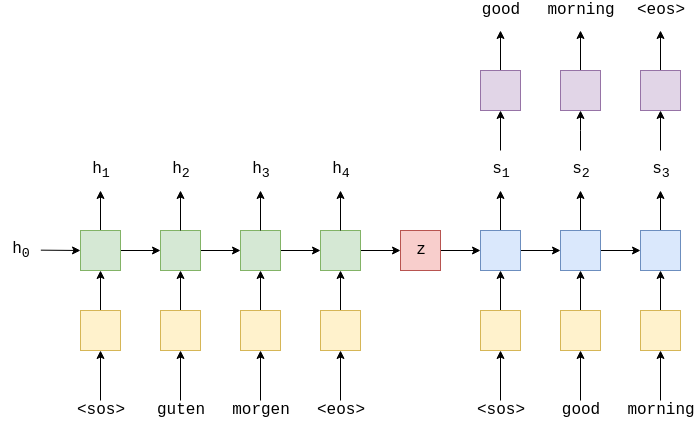
\includegraphics{assets/seq2seq1.png}
\caption{}
\end{figure}

The above image shows an example translation. The input/source sentence,
"guten morgen", is passed through the embedding layer (yellow) and then
input into the encoder (green). We also append a \emph{start of
sequence} (\texttt{\textless{}sos\textgreater{}}) and \emph{end of
sequence} (\texttt{\textless{}eos\textgreater{}}) token to the start and
end of sentence, respectively. At each time-step, the input to the
encoder RNN is both the embedding, \(e\), of the current word,
\(e(x_t)\), as well as the hidden state from the previous time-step,
\(h_{t-1}\), and the encoder RNN outputs a new hidden state \(h_t\). We
can think of the hidden state as a vector representation of the sentence
so far. The RNN can be represented as a function of both of \(e(x_t)\)
and \(h_{t-1}\):

\[h_t = \text{EncoderRNN}(e(x_t), h_{t-1})\]

We're using the term RNN generally here, it could be any recurrent
architecture, such as an \emph{LSTM} (Long Short-Term Memory) or a
\emph{GRU} (Gated Recurrent Unit).

Here, we have \(X = \{x_1, x_2, ..., x_T\}\), where
\(x_1 = \text{<sos>}, x_2 = \text{guten}\), etc. The initial hidden
state, \(h_0\), is usually either initialized to zeros or a learned
parameter.

Once the final word, \(x_T\), has been passed into the RNN via the
embedding layer, we use the final hidden state, \(h_T\), as the context
vector, i.e. \(h_T = z\). This is a vector representation of the entire
source sentence.

Now we have our context vector, \(z\), we can start decoding it to get
the output/target sentence, "good morning". Again, we append start and
end of sequence tokens to the target sentence. At each time-step, the
input to the decoder RNN (blue) is the embedding, \(d\), of current
word, \(d(y_t)\), as well as the hidden state from the previous
time-step, \(s_{t-1}\), where the initial decoder hidden state, \(s_0\),
is the context vector, \(s_0 = z = h_T\), i.e. the initial decoder
hidden state is the final encoder hidden state. Thus, similar to the
encoder, we can represent the decoder as:

\[s_t = \text{DecoderRNN}(d(y_t), s_{t-1})\]

Although the input/source embedding layer, \(e\), and the output/target
embedding layer, \(d\), are both shown in yellow in the diagram they are
two different embedding layers with their own parameters.

In the decoder, we need to go from the hidden state to an actual word,
therefore at each time-step we use \(s_t\) to predict (by passing it
through a \texttt{Linear} layer, shown in purple) what we think is the
next word in the sequence, \(\hat{y}_t\).

\[\hat{y}_t = f(s_t)\]

The words in the decoder are always generated one after another, with
one per time-step. We always use \texttt{\textless{}sos\textgreater{}}
for the first input to the decoder, \(y_1\), but for subsequent inputs,
\(y_{t>1}\), we will sometimes use the actual, ground truth next word in
the sequence, \(y_t\) and sometimes use the word predicted by our
decoder, \(\hat{y}_{t-1}\). This is called \emph{teacher forcing}, see a
bit more info about it
\href{https://machinelearningmastery.com/teacher-forcing-for-recurrent-neural-networks/}{here}.

When training/testing our model, we always know how many words are in
our target sentence, so we stop generating words once we hit that many.
During inference it is common to keep generating words until the model
outputs an \texttt{\textless{}eos\textgreater{}} token or after a
certain amount of words have been generated.

Once we have our predicted target sentence,
\(\hat{Y} = \{ \hat{y}_1, \hat{y}_2, ..., \hat{y}_T \}\), we compare it
against our actual target sentence, \(Y = \{ y_1, y_2, ..., y_T \}\), to
calculate our loss. We then use this loss to update all of the
parameters in our model.

\subsection{Preparing Data}\label{preparing-data}

We'll be coding up the models in PyTorch and using TorchText to help us
do all of the pre-processing required. We'll also be using spaCy to
assist in the tokenization of the data.

    \begin{Verbatim}[commandchars=\\\{\}]
{\color{incolor}In [{\color{incolor}1}]:} \PY{k+kn}{import} \PY{n+nn}{torch}
        \PY{k+kn}{import} \PY{n+nn}{torch}\PY{n+nn}{.}\PY{n+nn}{nn} \PY{k}{as} \PY{n+nn}{nn}
        \PY{k+kn}{import} \PY{n+nn}{torch}\PY{n+nn}{.}\PY{n+nn}{optim} \PY{k}{as} \PY{n+nn}{optim}
        
        \PY{k+kn}{from} \PY{n+nn}{torchtext}\PY{n+nn}{.}\PY{n+nn}{datasets} \PY{k}{import} \PY{n}{Multi30k}
        \PY{k+kn}{from} \PY{n+nn}{torchtext}\PY{n+nn}{.}\PY{n+nn}{data} \PY{k}{import} \PY{n}{Field}\PY{p}{,} \PY{n}{BucketIterator}
        
        \PY{k+kn}{import} \PY{n+nn}{spacy}
        \PY{k+kn}{import} \PY{n+nn}{numpy} \PY{k}{as} \PY{n+nn}{np}
        
        \PY{k+kn}{import} \PY{n+nn}{random}
        \PY{k+kn}{import} \PY{n+nn}{math}
        \PY{k+kn}{import} \PY{n+nn}{time}
        \PY{n+nb}{print}\PY{p}{(}\PY{n}{torch}\PY{o}{.}\PY{n}{\PYZus{}\PYZus{}version\PYZus{}\PYZus{}}\PY{p}{)}
\end{Verbatim}


    \begin{Verbatim}[commandchars=\\\{\}]
1.5.0

    \end{Verbatim}

    We'll set the random seeds for deterministic results.

    \begin{Verbatim}[commandchars=\\\{\}]
{\color{incolor}In [{\color{incolor}2}]:} \PY{n}{SEED} \PY{o}{=} \PY{l+m+mi}{1234}
        
        \PY{n}{random}\PY{o}{.}\PY{n}{seed}\PY{p}{(}\PY{n}{SEED}\PY{p}{)}
        \PY{n}{np}\PY{o}{.}\PY{n}{random}\PY{o}{.}\PY{n}{seed}\PY{p}{(}\PY{n}{SEED}\PY{p}{)}
        \PY{n}{torch}\PY{o}{.}\PY{n}{manual\PYZus{}seed}\PY{p}{(}\PY{n}{SEED}\PY{p}{)}
        \PY{n}{torch}\PY{o}{.}\PY{n}{cuda}\PY{o}{.}\PY{n}{manual\PYZus{}seed}\PY{p}{(}\PY{n}{SEED}\PY{p}{)}
        \PY{n}{torch}\PY{o}{.}\PY{n}{backends}\PY{o}{.}\PY{n}{cudnn}\PY{o}{.}\PY{n}{deterministic} \PY{o}{=} \PY{k+kc}{True}
\end{Verbatim}


    Next, we'll create the tokenizers. A tokenizer is used to turn a string
containing a sentence into a list of individual tokens that make up that
string, e.g. "good morning!" becomes {[}"good", "morning", "!"{]}. We'll
start talking about the sentences being a sequence of tokens from now,
instead of saying they're a sequence of words. What's the difference?
Well, "good" and "morning" are both words and tokens, but "!" is a
token, not a word.

spaCy has model for each language ("de" for German and "en" for English)
which need to be loaded so we can access the tokenizer of each model.

\textbf{Note}: the models must first be downloaded using the following
on the command line:

\begin{verbatim}
python -m spacy download en
python -m spacy download de
\end{verbatim}

We load the models as such:

    \begin{Verbatim}[commandchars=\\\{\}]
{\color{incolor}In [{\color{incolor}4}]:} \PY{n}{spacy\PYZus{}de} \PY{o}{=} \PY{n}{spacy}\PY{o}{.}\PY{n}{load}\PY{p}{(}\PY{l+s+s1}{\PYZsq{}}\PY{l+s+s1}{de\PYZus{}core\PYZus{}news\PYZus{}sm}\PY{l+s+s1}{\PYZsq{}}\PY{p}{)}
        \PY{n}{spacy\PYZus{}en} \PY{o}{=} \PY{n}{spacy}\PY{o}{.}\PY{n}{load}\PY{p}{(}\PY{l+s+s1}{\PYZsq{}}\PY{l+s+s1}{en\PYZus{}core\PYZus{}web\PYZus{}sm}\PY{l+s+s1}{\PYZsq{}}\PY{p}{)}
\end{Verbatim}


    Next, we create the tokenizer functions. These can be passed to
TorchText and will take in the sentence as a string and return the
sentence as a list of tokens.

In the paper we are implementing, they find it beneficial to reverse the
order of the input which they believe "introduces many short term
dependencies in the data that make the optimization problem much
easier". We copy this by reversing the German sentence after it has been
transformed into a list of tokens.

    \begin{Verbatim}[commandchars=\\\{\}]
{\color{incolor}In [{\color{incolor}5}]:} \PY{k}{def} \PY{n+nf}{tokenize\PYZus{}de}\PY{p}{(}\PY{n}{text}\PY{p}{)}\PY{p}{:}
            \PY{l+s+sd}{\PYZdq{}\PYZdq{}\PYZdq{}}
        \PY{l+s+sd}{    Tokenizes German text from a string into a list of strings (tokens) and reverses it}
        \PY{l+s+sd}{    \PYZdq{}\PYZdq{}\PYZdq{}}
            \PY{k}{return} \PY{p}{[}\PY{n}{tok}\PY{o}{.}\PY{n}{text} \PY{k}{for} \PY{n}{tok} \PY{o+ow}{in} \PY{n}{spacy\PYZus{}de}\PY{o}{.}\PY{n}{tokenizer}\PY{p}{(}\PY{n}{text}\PY{p}{)}\PY{p}{]}\PY{p}{[}\PY{p}{:}\PY{p}{:}\PY{o}{\PYZhy{}}\PY{l+m+mi}{1}\PY{p}{]}
        
        \PY{k}{def} \PY{n+nf}{tokenize\PYZus{}en}\PY{p}{(}\PY{n}{text}\PY{p}{)}\PY{p}{:}
            \PY{l+s+sd}{\PYZdq{}\PYZdq{}\PYZdq{}}
        \PY{l+s+sd}{    Tokenizes English text from a string into a list of strings (tokens)}
        \PY{l+s+sd}{    \PYZdq{}\PYZdq{}\PYZdq{}}
            \PY{k}{return} \PY{p}{[}\PY{n}{tok}\PY{o}{.}\PY{n}{text} \PY{k}{for} \PY{n}{tok} \PY{o+ow}{in} \PY{n}{spacy\PYZus{}en}\PY{o}{.}\PY{n}{tokenizer}\PY{p}{(}\PY{n}{text}\PY{p}{)}\PY{p}{]}
\end{Verbatim}


    TorchText's \texttt{Field}s handle how data should be processed. All of
the possible arguments are detailed
\href{https://github.com/pytorch/text/blob/master/torchtext/data/field.py\#L61}{here}.

We set the \texttt{tokenize} argument to the correct tokenization
function for each, with German being the \texttt{SRC} (source) field and
English being the \texttt{TRG} (target) field. The field also appends
the "start of sequence" and "end of sequence" tokens via the
\texttt{init\_token} and \texttt{eos\_token} arguments, and converts all
words to lowercase.

    \begin{Verbatim}[commandchars=\\\{\}]
{\color{incolor}In [{\color{incolor}6}]:} \PY{n}{SRC} \PY{o}{=} \PY{n}{Field}\PY{p}{(}\PY{n}{tokenize} \PY{o}{=} \PY{n}{tokenize\PYZus{}de}\PY{p}{,} 
                    \PY{n}{init\PYZus{}token} \PY{o}{=} \PY{l+s+s1}{\PYZsq{}}\PY{l+s+s1}{\PYZlt{}sos\PYZgt{}}\PY{l+s+s1}{\PYZsq{}}\PY{p}{,} 
                    \PY{n}{eos\PYZus{}token} \PY{o}{=} \PY{l+s+s1}{\PYZsq{}}\PY{l+s+s1}{\PYZlt{}eos\PYZgt{}}\PY{l+s+s1}{\PYZsq{}}\PY{p}{,} 
                    \PY{n}{lower} \PY{o}{=} \PY{k+kc}{True}\PY{p}{)}
        
        \PY{n}{TRG} \PY{o}{=} \PY{n}{Field}\PY{p}{(}\PY{n}{tokenize} \PY{o}{=} \PY{n}{tokenize\PYZus{}en}\PY{p}{,} 
                    \PY{n}{init\PYZus{}token} \PY{o}{=} \PY{l+s+s1}{\PYZsq{}}\PY{l+s+s1}{\PYZlt{}sos\PYZgt{}}\PY{l+s+s1}{\PYZsq{}}\PY{p}{,} 
                    \PY{n}{eos\PYZus{}token} \PY{o}{=} \PY{l+s+s1}{\PYZsq{}}\PY{l+s+s1}{\PYZlt{}eos\PYZgt{}}\PY{l+s+s1}{\PYZsq{}}\PY{p}{,} 
                    \PY{n}{lower} \PY{o}{=} \PY{k+kc}{True}\PY{p}{)}
\end{Verbatim}


    Next, we download and load the train, validation and test data.

The dataset we'll be using is the
\href{https://github.com/multi30k/dataset}{Multi30k dataset}. This is a
dataset with \textasciitilde{}30,000 parallel English, German and French
sentences, each with \textasciitilde{}12 words per sentence.

\texttt{exts} specifies which languages to use as the source and target
(source goes first) and \texttt{fields} specifies which field to use for
the source and target.

    \begin{Verbatim}[commandchars=\\\{\}]
{\color{incolor}In [{\color{incolor}7}]:} \PY{n}{train\PYZus{}data}\PY{p}{,} \PY{n}{valid\PYZus{}data}\PY{p}{,} \PY{n}{test\PYZus{}data} \PY{o}{=} \PY{n}{Multi30k}\PY{o}{.}\PY{n}{splits}\PY{p}{(}\PY{n}{exts} \PY{o}{=} \PY{p}{(}\PY{l+s+s1}{\PYZsq{}}\PY{l+s+s1}{.de}\PY{l+s+s1}{\PYZsq{}}\PY{p}{,} \PY{l+s+s1}{\PYZsq{}}\PY{l+s+s1}{.en}\PY{l+s+s1}{\PYZsq{}}\PY{p}{)}\PY{p}{,} 
                                                            \PY{n}{fields} \PY{o}{=} \PY{p}{(}\PY{n}{SRC}\PY{p}{,} \PY{n}{TRG}\PY{p}{)}\PY{p}{)}
\end{Verbatim}


    \begin{Verbatim}[commandchars=\\\{\}]
downloading training.tar.gz

    \end{Verbatim}

    \begin{Verbatim}[commandchars=\\\{\}]
training.tar.gz: 100\%|██████████| 1.21M/1.21M [00:04<00:00, 286kB/s] 

    \end{Verbatim}

    \begin{Verbatim}[commandchars=\\\{\}]
downloading validation.tar.gz

    \end{Verbatim}

    \begin{Verbatim}[commandchars=\\\{\}]
validation.tar.gz: 100\%|██████████| 46.3k/46.3k [00:00<00:00, 53.9kB/s]

    \end{Verbatim}

    \begin{Verbatim}[commandchars=\\\{\}]
downloading mmt\_task1\_test2016.tar.gz

    \end{Verbatim}

    \begin{Verbatim}[commandchars=\\\{\}]
mmt\_task1\_test2016.tar.gz: 100\%|██████████| 66.2k/66.2k [00:00<00:00, 76.5kB/s]

    \end{Verbatim}

    We can double check that we've loaded the right number of examples:

    \begin{Verbatim}[commandchars=\\\{\}]
{\color{incolor}In [{\color{incolor}8}]:} \PY{n+nb}{print}\PY{p}{(}\PY{n}{f}\PY{l+s+s2}{\PYZdq{}}\PY{l+s+s2}{Number of training examples: }\PY{l+s+s2}{\PYZob{}}\PY{l+s+s2}{len(train\PYZus{}data.examples)\PYZcb{}}\PY{l+s+s2}{\PYZdq{}}\PY{p}{)}
        \PY{n+nb}{print}\PY{p}{(}\PY{n}{f}\PY{l+s+s2}{\PYZdq{}}\PY{l+s+s2}{Number of validation examples: }\PY{l+s+s2}{\PYZob{}}\PY{l+s+s2}{len(valid\PYZus{}data.examples)\PYZcb{}}\PY{l+s+s2}{\PYZdq{}}\PY{p}{)}
        \PY{n+nb}{print}\PY{p}{(}\PY{n}{f}\PY{l+s+s2}{\PYZdq{}}\PY{l+s+s2}{Number of testing examples: }\PY{l+s+s2}{\PYZob{}}\PY{l+s+s2}{len(test\PYZus{}data.examples)\PYZcb{}}\PY{l+s+s2}{\PYZdq{}}\PY{p}{)}
\end{Verbatim}


    \begin{Verbatim}[commandchars=\\\{\}]
Number of training examples: 29000
Number of validation examples: 1014
Number of testing examples: 1000

    \end{Verbatim}

    We can also print out an example, making sure the source sentence is
reversed:

    \begin{Verbatim}[commandchars=\\\{\}]
{\color{incolor}In [{\color{incolor}9}]:} \PY{n+nb}{print}\PY{p}{(}\PY{n+nb}{vars}\PY{p}{(}\PY{n}{train\PYZus{}data}\PY{o}{.}\PY{n}{examples}\PY{p}{[}\PY{l+m+mi}{0}\PY{p}{]}\PY{p}{)}\PY{p}{)}
\end{Verbatim}


    \begin{Verbatim}[commandchars=\\\{\}]
\{'src': ['.', 'büsche', 'vieler', 'nähe', 'der', 'in', 'freien', 'im', 'sind', 'männer', 'weiße', 'junge', 'zwei'], 'trg': ['two', 'young', ',', 'white', 'males', 'are', 'outside', 'near', 'many', 'bushes', '.']\}

    \end{Verbatim}

    The period is at the beginning of the German (src) sentence, so it looks
like the sentence has been correctly reversed.

Next, we'll build the \emph{vocabulary} for the source and target
languages. The vocabulary is used to associate each unique token with an
index (an integer). The vocabularies of the source and target languages
are distinct.

Using the \texttt{min\_freq} argument, we only allow tokens that appear
at least 2 times to appear in our vocabulary. Tokens that appear only
once are converted into an \texttt{\textless{}unk\textgreater{}}
(unknown) token.

It is important to note that our vocabulary should only be built from
the training set and not the validation/test set. This prevents
"information leakage" into our model, giving us artifically inflated
validation/test scores.

    \begin{Verbatim}[commandchars=\\\{\}]
{\color{incolor}In [{\color{incolor}10}]:} \PY{n}{SRC}\PY{o}{.}\PY{n}{build\PYZus{}vocab}\PY{p}{(}\PY{n}{train\PYZus{}data}\PY{p}{,} \PY{n}{min\PYZus{}freq} \PY{o}{=} \PY{l+m+mi}{2}\PY{p}{)}
         \PY{n}{TRG}\PY{o}{.}\PY{n}{build\PYZus{}vocab}\PY{p}{(}\PY{n}{train\PYZus{}data}\PY{p}{,} \PY{n}{min\PYZus{}freq} \PY{o}{=} \PY{l+m+mi}{2}\PY{p}{)}
\end{Verbatim}


    \begin{Verbatim}[commandchars=\\\{\}]
{\color{incolor}In [{\color{incolor}11}]:} \PY{n+nb}{print}\PY{p}{(}\PY{n}{f}\PY{l+s+s2}{\PYZdq{}}\PY{l+s+s2}{Unique tokens in source (de) vocabulary: }\PY{l+s+s2}{\PYZob{}}\PY{l+s+s2}{len(SRC.vocab)\PYZcb{}}\PY{l+s+s2}{\PYZdq{}}\PY{p}{)}
         \PY{n+nb}{print}\PY{p}{(}\PY{n}{f}\PY{l+s+s2}{\PYZdq{}}\PY{l+s+s2}{Unique tokens in target (en) vocabulary: }\PY{l+s+s2}{\PYZob{}}\PY{l+s+s2}{len(TRG.vocab)\PYZcb{}}\PY{l+s+s2}{\PYZdq{}}\PY{p}{)}
\end{Verbatim}


    \begin{Verbatim}[commandchars=\\\{\}]
Unique tokens in source (de) vocabulary: 7854
Unique tokens in target (en) vocabulary: 5893

    \end{Verbatim}

    The final step of preparing the data is to create the iterators. These
can be iterated on to return a batch of data which will have a
\texttt{src} attribute (the PyTorch tensors containing a batch of
numericalized source sentences) and a \texttt{trg} attribute (the
PyTorch tensors containing a batch of numericalized target sentences).
Numericalized is just a fancy way of saying they have been converted
from a sequence of readable tokens to a sequence of corresponding
indexes, using the vocabulary.

We also need to define a \texttt{torch.device}. This is used to tell
TorchText to put the tensors on the GPU or not. We use the
\texttt{torch.cuda.is\_available()} function, which will return
\texttt{True} if a GPU is detected on our computer. We pass this
\texttt{device} to the iterator.

When we get a batch of examples using an iterator we need to make sure
that all of the source sentences are padded to the same length, the same
with the target sentences. Luckily, TorchText iterators handle this for
us!

We use a \texttt{BucketIterator} instead of the standard
\texttt{Iterator} as it creates batches in such a way that it minimizes
the amount of padding in both the source and target sentences.

    \begin{Verbatim}[commandchars=\\\{\}]
{\color{incolor}In [{\color{incolor}12}]:} \PY{n}{device} \PY{o}{=} \PY{n}{torch}\PY{o}{.}\PY{n}{device}\PY{p}{(}\PY{l+s+s1}{\PYZsq{}}\PY{l+s+s1}{cuda}\PY{l+s+s1}{\PYZsq{}} \PY{k}{if} \PY{n}{torch}\PY{o}{.}\PY{n}{cuda}\PY{o}{.}\PY{n}{is\PYZus{}available}\PY{p}{(}\PY{p}{)} \PY{k}{else} \PY{l+s+s1}{\PYZsq{}}\PY{l+s+s1}{cpu}\PY{l+s+s1}{\PYZsq{}}\PY{p}{)}
\end{Verbatim}


    \begin{Verbatim}[commandchars=\\\{\}]
{\color{incolor}In [{\color{incolor}13}]:} \PY{n}{BATCH\PYZus{}SIZE} \PY{o}{=} \PY{l+m+mi}{128}
         
         \PY{n}{train\PYZus{}iterator}\PY{p}{,} \PY{n}{valid\PYZus{}iterator}\PY{p}{,} \PY{n}{test\PYZus{}iterator} \PY{o}{=} \PY{n}{BucketIterator}\PY{o}{.}\PY{n}{splits}\PY{p}{(}
             \PY{p}{(}\PY{n}{train\PYZus{}data}\PY{p}{,} \PY{n}{valid\PYZus{}data}\PY{p}{,} \PY{n}{test\PYZus{}data}\PY{p}{)}\PY{p}{,} 
             \PY{n}{batch\PYZus{}size} \PY{o}{=} \PY{n}{BATCH\PYZus{}SIZE}\PY{p}{,} 
             \PY{n}{device} \PY{o}{=} \PY{n}{device}\PY{p}{)}
\end{Verbatim}


    \subsection{Building the Seq2Seq
Model}\label{building-the-seq2seq-model}

We'll be building our model in three parts. The encoder, the decoder and
a seq2seq model that encapsulates the encoder and decoder and will
provide a way to interface with each.

\subsubsection{Encoder}\label{encoder}

First, the encoder, a 2 layer LSTM. The paper we are implementing uses a
4-layer LSTM, but in the interest of training time we cut this down to
2-layers. The concept of multi-layer RNNs is easy to expand from 2 to 4
layers.

For a multi-layer RNN, the input sentence, \(X\), after being embedded
goes into the first (bottom) layer of the RNN and hidden states,
\(H=\{h_1, h_2, ..., h_T\}\), output by this layer are used as inputs to
the RNN in the layer above. Thus, representing each layer with a
superscript, the hidden states in the first layer are given by:

\[h_t^1 = \text{EncoderRNN}^1(e(x_t), h_{t-1}^1)\]

The hidden states in the second layer are given by:

\[h_t^2 = \text{EncoderRNN}^2(h_t^1, h_{t-1}^2)\]

Using a multi-layer RNN also means we'll also need an initial hidden
state as input per layer, \(h_0^l\), and we will also output a context
vector per layer, \(z^l\).

Without going into too much detail about LSTMs (see
\href{https://colah.github.io/posts/2015-08-Understanding-LSTMs/}{this}
blog post to learn more about them), all we need to know is that they're
a type of RNN which instead of just taking in a hidden state and
returning a new hidden state per time-step, also take in and return a
\emph{cell state}, \(c_t\), per time-step.

\[\begin{align*}
h_t &= \text{RNN}(e(x_t), h_{t-1})\\
(h_t, c_t) &= \text{LSTM}(e(x_t), h_{t-1}, c_{t-1})
\end{align*}\]

We can just think of \(c_t\) as another type of hidden state. Similar to
\(h_0^l\), \(c_0^l\) will be initialized to a tensor of all zeros. Also,
our context vector will now be both the final hidden state and the final
cell state, i.e. \(z^l = (h_T^l, c_T^l)\).

Extending our multi-layer equations to LSTMs, we get:

\[\begin{align*}
(h_t^1, c_t^1) &= \text{EncoderLSTM}^1(e(x_t), (h_{t-1}^1, c_{t-1}^1))\\
(h_t^2, c_t^2) &= \text{EncoderLSTM}^2(h_t^1, (h_{t-1}^2, c_{t-1}^2))
\end{align*}\]

Note how only our hidden state from the first layer is passed as input
to the second layer, and not the cell state.

So our encoder looks something like this:

\begin{figure}
\centering
\includegraphics{assets/seq2seq2.png}
\caption{}
\end{figure}

We create this in code by making an \texttt{Encoder} module, which
requires we inherit from \texttt{torch.nn.Module} and use the
\texttt{super().\_\_init\_\_()} as some boilerplate code. The encoder
takes the following arguments: - \texttt{input\_dim} is the
size/dimensionality of the one-hot vectors that will be input to the
encoder. This is equal to the input (source) vocabulary size. -
\texttt{emb\_dim} is the dimensionality of the embedding layer. This
layer converts the one-hot vectors into dense vectors with
\texttt{emb\_dim} dimensions. - \texttt{hid\_dim} is the dimensionality
of the hidden and cell states. - \texttt{n\_layers} is the number of
layers in the RNN. - \texttt{dropout} is the amount of dropout to use.
This is a regularization parameter to prevent overfitting. Check out
\href{https://www.coursera.org/lecture/deep-neural-network/understanding-dropout-YaGbR}{this}
for more details about dropout.

We aren't going to discuss the embedding layer in detail during these
tutorials. All we need to know is that there is a step before the words
- technically, the indexes of the words - are passed into the RNN, where
the words are transformed into vectors. To read more about word
embeddings, check these articles:
\href{https://monkeylearn.com/blog/word-embeddings-transform-text-numbers/}{1},
\href{http://p.migdal.pl/2017/01/06/king-man-woman-queen-why.html}{2},
\href{http://mccormickml.com/2016/04/19/word2vec-tutorial-the-skip-gram-model/}{3},
\href{http://mccormickml.com/2017/01/11/word2vec-tutorial-part-2-negative-sampling/}{4}.

The embedding layer is created using \texttt{nn.Embedding}, the LSTM
with \texttt{nn.LSTM} and a dropout layer with \texttt{nn.Dropout}.
Check the PyTorch
\href{https://pytorch.org/docs/stable/nn.html}{documentation} for more
about these.

One thing to note is that the \texttt{dropout} argument to the LSTM is
how much dropout to apply between the layers of a multi-layer RNN, i.e.
between the hidden states output from layer \(l\) and those same hidden
states being used for the input of layer \(l+1\).

In the \texttt{forward} method, we pass in the source sentence, \(X\),
which is converted into dense vectors using the \texttt{embedding}
layer, and then dropout is applied. These embeddings are then passed
into the RNN. As we pass a whole sequence to the RNN, it will
automatically do the recurrent calculation of the hidden states over the
whole sequence for us! Notice that we do not pass an initial hidden or
cell state to the RNN. This is because, as noted in the
\href{https://pytorch.org/docs/stable/nn.html\#torch.nn.LSTM}{documentation},
that if no hidden/cell state is passed to the RNN, it will automatically
create an initial hidden/cell state as a tensor of all zeros.

The RNN returns: \texttt{outputs} (the top-layer hidden state for each
time-step), \texttt{hidden} (the final hidden state for each layer,
\(h_T\), stacked on top of each other) and \texttt{cell} (the final cell
state for each layer, \(c_T\), stacked on top of each other).

As we only need the final hidden and cell states (to make our context
vector), \texttt{forward} only returns \texttt{hidden} and
\texttt{cell}.

The sizes of each of the tensors is left as comments in the code. In
this implementation \texttt{n\_directions} will always be 1, however
note that bidirectional RNNs (covered in tutorial 3) will have
\texttt{n\_directions} as 2.

    \begin{Verbatim}[commandchars=\\\{\}]
{\color{incolor}In [{\color{incolor}14}]:} \PY{k}{class} \PY{n+nc}{Encoder}\PY{p}{(}\PY{n}{nn}\PY{o}{.}\PY{n}{Module}\PY{p}{)}\PY{p}{:}
             \PY{k}{def} \PY{n+nf}{\PYZus{}\PYZus{}init\PYZus{}\PYZus{}}\PY{p}{(}\PY{n+nb+bp}{self}\PY{p}{,} \PY{n}{input\PYZus{}dim}\PY{p}{,} \PY{n}{emb\PYZus{}dim}\PY{p}{,} \PY{n}{hid\PYZus{}dim}\PY{p}{,} \PY{n}{n\PYZus{}layers}\PY{p}{,} \PY{n}{dropout}\PY{p}{)}\PY{p}{:}
                 \PY{n+nb}{super}\PY{p}{(}\PY{p}{)}\PY{o}{.}\PY{n+nf+fm}{\PYZus{}\PYZus{}init\PYZus{}\PYZus{}}\PY{p}{(}\PY{p}{)}
                 
                 \PY{n+nb+bp}{self}\PY{o}{.}\PY{n}{hid\PYZus{}dim} \PY{o}{=} \PY{n}{hid\PYZus{}dim}
                 \PY{n+nb+bp}{self}\PY{o}{.}\PY{n}{n\PYZus{}layers} \PY{o}{=} \PY{n}{n\PYZus{}layers}
                 
                 \PY{n+nb+bp}{self}\PY{o}{.}\PY{n}{embedding} \PY{o}{=} \PY{n}{nn}\PY{o}{.}\PY{n}{Embedding}\PY{p}{(}\PY{n}{input\PYZus{}dim}\PY{p}{,} \PY{n}{emb\PYZus{}dim}\PY{p}{)}
                 
                 \PY{n+nb+bp}{self}\PY{o}{.}\PY{n}{rnn} \PY{o}{=} \PY{n}{nn}\PY{o}{.}\PY{n}{LSTM}\PY{p}{(}\PY{n}{emb\PYZus{}dim}\PY{p}{,} \PY{n}{hid\PYZus{}dim}\PY{p}{,} \PY{n}{n\PYZus{}layers}\PY{p}{,} \PY{n}{dropout} \PY{o}{=} \PY{n}{dropout}\PY{p}{)}
                 
                 \PY{n+nb+bp}{self}\PY{o}{.}\PY{n}{dropout} \PY{o}{=} \PY{n}{nn}\PY{o}{.}\PY{n}{Dropout}\PY{p}{(}\PY{n}{dropout}\PY{p}{)}
                 
             \PY{k}{def} \PY{n+nf}{forward}\PY{p}{(}\PY{n+nb+bp}{self}\PY{p}{,} \PY{n}{src}\PY{p}{)}\PY{p}{:}
                 
                 \PY{c+c1}{\PYZsh{}src = [src len, batch size]}
                 
                 \PY{n}{embedded} \PY{o}{=} \PY{n+nb+bp}{self}\PY{o}{.}\PY{n}{dropout}\PY{p}{(}\PY{n+nb+bp}{self}\PY{o}{.}\PY{n}{embedding}\PY{p}{(}\PY{n}{src}\PY{p}{)}\PY{p}{)}
                 
                 \PY{c+c1}{\PYZsh{}embedded = [src len, batch size, emb dim]}
                 
                 \PY{n}{outputs}\PY{p}{,} \PY{p}{(}\PY{n}{hidden}\PY{p}{,} \PY{n}{cell}\PY{p}{)} \PY{o}{=} \PY{n+nb+bp}{self}\PY{o}{.}\PY{n}{rnn}\PY{p}{(}\PY{n}{embedded}\PY{p}{)}
                 
                 \PY{c+c1}{\PYZsh{}outputs = [src len, batch size, hid dim * n directions]}
                 \PY{c+c1}{\PYZsh{}hidden = [n layers * n directions, batch size, hid dim]}
                 \PY{c+c1}{\PYZsh{}cell = [n layers * n directions, batch size, hid dim]}
                 
                 \PY{c+c1}{\PYZsh{}outputs are always from the top hidden layer}
                 
                 \PY{k}{return} \PY{n}{hidden}\PY{p}{,} \PY{n}{cell}
\end{Verbatim}


    \subsubsection{Decoder}\label{decoder}

Next, we'll build our decoder, which will also be a 2-layer (4 in the
paper) LSTM.

\begin{figure}
\centering
\includegraphics{assets/seq2seq3.png}
\caption{}
\end{figure}

The \texttt{Decoder} class does a single step of decoding, i.e. it
ouputs single token per time-step. The first layer will receive a hidden
and cell state from the previous time-step, \((s_{t-1}^1, c_{t-1}^1)\),
and feeds it through the LSTM with the current embedded token, \(y_t\),
to produce a new hidden and cell state, \((s_t^1, c_t^1)\). The
subsequent layers will use the hidden state from the layer below,
\(s_t^{l-1}\), and the previous hidden and cell states from their layer,
\((s_{t-1}^l, c_{t-1}^l)\). This provides equations very similar to
those in the encoder.

\[\begin{align*}
(s_t^1, c_t^1) = \text{DecoderLSTM}^1(d(y_t), (s_{t-1}^1, c_{t-1}^1))\\
(s_t^2, c_t^2) = \text{DecoderLSTM}^2(s_t^1, (s_{t-1}^2, c_{t-1}^2))
\end{align*}\]

Remember that the initial hidden and cell states to our decoder are our
context vectors, which are the final hidden and cell states of our
encoder from the same layer, i.e. \((s_0^l,c_0^l)=z^l=(h_T^l,c_T^l)\).

We then pass the hidden state from the top layer of the RNN, \(s_t^L\),
through a linear layer, \(f\), to make a prediction of what the next
token in the target (output) sequence should be, \(\hat{y}_{t+1}\).

\[\hat{y}_{t+1} = f(s_t^L)\]

The arguments and initialization are similar to the \texttt{Encoder}
class, except we now have an \texttt{output\_dim} which is the size of
the vocabulary for the output/target. There is also the addition of the
\texttt{Linear} layer, used to make the predictions from the top layer
hidden state.

Within the \texttt{forward} method, we accept a batch of input tokens,
previous hidden states and previous cell states. As we are only decoding
one token at a time, the input tokens will always have a sequence length
of 1. We \texttt{unsqueeze} the input tokens to add a sentence length
dimension of 1. Then, similar to the encoder, we pass through an
embedding layer and apply dropout. This batch of embedded tokens is then
passed into the RNN with the previous hidden and cell states. This
produces an \texttt{output} (hidden state from the top layer of the
RNN), a new \texttt{hidden} state (one for each layer, stacked on top of
each other) and a new \texttt{cell} state (also one per layer, stacked
on top of each other). We then pass the \texttt{output} (after getting
rid of the sentence length dimension) through the linear layer to
receive our \texttt{prediction}. We then return the \texttt{prediction},
the new \texttt{hidden} state and the new \texttt{cell} state.

\textbf{Note}: as we always have a sequence length of 1, we could use
\texttt{nn.LSTMCell}, instead of \texttt{nn.LSTM}, as it is designed to
handle a batch of inputs that aren't necessarily in a sequence.
\texttt{nn.LSTMCell} is just a single cell and \texttt{nn.LSTM} is a
wrapper around potentially multiple cells. Using the
\texttt{nn.LSTMCell} in this case would mean we don't have to
\texttt{unsqueeze} to add a fake sequence length dimension, but we would
need one \texttt{nn.LSTMCell} per layer in the decoder and to ensure
each \texttt{nn.LSTMCell} receives the correct initial hidden state from
the encoder. All of this makes the code less concise - hence the
decision to stick with the regular \texttt{nn.LSTM}.

    \begin{Verbatim}[commandchars=\\\{\}]
{\color{incolor}In [{\color{incolor}15}]:} \PY{k}{class} \PY{n+nc}{Decoder}\PY{p}{(}\PY{n}{nn}\PY{o}{.}\PY{n}{Module}\PY{p}{)}\PY{p}{:}
             \PY{k}{def} \PY{n+nf}{\PYZus{}\PYZus{}init\PYZus{}\PYZus{}}\PY{p}{(}\PY{n+nb+bp}{self}\PY{p}{,} \PY{n}{output\PYZus{}dim}\PY{p}{,} \PY{n}{emb\PYZus{}dim}\PY{p}{,} \PY{n}{hid\PYZus{}dim}\PY{p}{,} \PY{n}{n\PYZus{}layers}\PY{p}{,} \PY{n}{dropout}\PY{p}{)}\PY{p}{:}
                 \PY{n+nb}{super}\PY{p}{(}\PY{p}{)}\PY{o}{.}\PY{n+nf+fm}{\PYZus{}\PYZus{}init\PYZus{}\PYZus{}}\PY{p}{(}\PY{p}{)}
                 
                 \PY{n+nb+bp}{self}\PY{o}{.}\PY{n}{output\PYZus{}dim} \PY{o}{=} \PY{n}{output\PYZus{}dim}
                 \PY{n+nb+bp}{self}\PY{o}{.}\PY{n}{hid\PYZus{}dim} \PY{o}{=} \PY{n}{hid\PYZus{}dim}
                 \PY{n+nb+bp}{self}\PY{o}{.}\PY{n}{n\PYZus{}layers} \PY{o}{=} \PY{n}{n\PYZus{}layers}
                 
                 \PY{n+nb+bp}{self}\PY{o}{.}\PY{n}{embedding} \PY{o}{=} \PY{n}{nn}\PY{o}{.}\PY{n}{Embedding}\PY{p}{(}\PY{n}{output\PYZus{}dim}\PY{p}{,} \PY{n}{emb\PYZus{}dim}\PY{p}{)}
                 
                 \PY{n+nb+bp}{self}\PY{o}{.}\PY{n}{rnn} \PY{o}{=} \PY{n}{nn}\PY{o}{.}\PY{n}{LSTM}\PY{p}{(}\PY{n}{emb\PYZus{}dim}\PY{p}{,} \PY{n}{hid\PYZus{}dim}\PY{p}{,} \PY{n}{n\PYZus{}layers}\PY{p}{,} \PY{n}{dropout} \PY{o}{=} \PY{n}{dropout}\PY{p}{)}
                 
                 \PY{n+nb+bp}{self}\PY{o}{.}\PY{n}{fc\PYZus{}out} \PY{o}{=} \PY{n}{nn}\PY{o}{.}\PY{n}{Linear}\PY{p}{(}\PY{n}{hid\PYZus{}dim}\PY{p}{,} \PY{n}{output\PYZus{}dim}\PY{p}{)}
                 
                 \PY{n+nb+bp}{self}\PY{o}{.}\PY{n}{dropout} \PY{o}{=} \PY{n}{nn}\PY{o}{.}\PY{n}{Dropout}\PY{p}{(}\PY{n}{dropout}\PY{p}{)}
                 
             \PY{k}{def} \PY{n+nf}{forward}\PY{p}{(}\PY{n+nb+bp}{self}\PY{p}{,} \PY{n+nb}{input}\PY{p}{,} \PY{n}{hidden}\PY{p}{,} \PY{n}{cell}\PY{p}{)}\PY{p}{:}
                 
                 \PY{c+c1}{\PYZsh{}input = [batch size]}
                 \PY{c+c1}{\PYZsh{}hidden = [n layers * n directions, batch size, hid dim]}
                 \PY{c+c1}{\PYZsh{}cell = [n layers * n directions, batch size, hid dim]}
                 
                 \PY{c+c1}{\PYZsh{}n directions in the decoder will both always be 1, therefore:}
                 \PY{c+c1}{\PYZsh{}hidden = [n layers, batch size, hid dim]}
                 \PY{c+c1}{\PYZsh{}context = [n layers, batch size, hid dim]}
                 
                 \PY{n+nb}{input} \PY{o}{=} \PY{n+nb}{input}\PY{o}{.}\PY{n}{unsqueeze}\PY{p}{(}\PY{l+m+mi}{0}\PY{p}{)}
                 
                 \PY{c+c1}{\PYZsh{}input = [1, batch size]}
                 
                 \PY{n}{embedded} \PY{o}{=} \PY{n+nb+bp}{self}\PY{o}{.}\PY{n}{dropout}\PY{p}{(}\PY{n+nb+bp}{self}\PY{o}{.}\PY{n}{embedding}\PY{p}{(}\PY{n+nb}{input}\PY{p}{)}\PY{p}{)}
                 
                 \PY{c+c1}{\PYZsh{}embedded = [1, batch size, emb dim]}
                         
                 \PY{n}{output}\PY{p}{,} \PY{p}{(}\PY{n}{hidden}\PY{p}{,} \PY{n}{cell}\PY{p}{)} \PY{o}{=} \PY{n+nb+bp}{self}\PY{o}{.}\PY{n}{rnn}\PY{p}{(}\PY{n}{embedded}\PY{p}{,} \PY{p}{(}\PY{n}{hidden}\PY{p}{,} \PY{n}{cell}\PY{p}{)}\PY{p}{)}
                 
                 \PY{c+c1}{\PYZsh{}output = [seq len, batch size, hid dim * n directions]}
                 \PY{c+c1}{\PYZsh{}hidden = [n layers * n directions, batch size, hid dim]}
                 \PY{c+c1}{\PYZsh{}cell = [n layers * n directions, batch size, hid dim]}
                 
                 \PY{c+c1}{\PYZsh{}seq len and n directions will always be 1 in the decoder, therefore:}
                 \PY{c+c1}{\PYZsh{}output = [1, batch size, hid dim]}
                 \PY{c+c1}{\PYZsh{}hidden = [n layers, batch size, hid dim]}
                 \PY{c+c1}{\PYZsh{}cell = [n layers, batch size, hid dim]}
                 
                 \PY{n}{prediction} \PY{o}{=} \PY{n+nb+bp}{self}\PY{o}{.}\PY{n}{fc\PYZus{}out}\PY{p}{(}\PY{n}{output}\PY{o}{.}\PY{n}{squeeze}\PY{p}{(}\PY{l+m+mi}{0}\PY{p}{)}\PY{p}{)}
                 
                 \PY{c+c1}{\PYZsh{}prediction = [batch size, output dim]}
                 
                 \PY{k}{return} \PY{n}{prediction}\PY{p}{,} \PY{n}{hidden}\PY{p}{,} \PY{n}{cell}
\end{Verbatim}


    \subsubsection{Seq2Seq}\label{seq2seq}

For the final part of the implemenetation, we'll implement the seq2seq
model. This will handle: - receiving the input/source sentence - using
the encoder to produce the context vectors - using the decoder to
produce the predicted output/target sentence

Our full model will look like this:

\begin{figure}
\centering
\includegraphics{assets/seq2seq4.png}
\caption{}
\end{figure}

The \texttt{Seq2Seq} model takes in an \texttt{Encoder},
\texttt{Decoder}, and a \texttt{device} (used to place tensors on the
GPU, if it exists).

For this implementation, we have to ensure that the number of layers and
the hidden (and cell) dimensions are equal in the \texttt{Encoder} and
\texttt{Decoder}. This is not always the case, we do not necessarily
need the same number of layers or the same hidden dimension sizes in a
sequence-to-sequence model. However, if we did something like having a
different number of layers then we would need to make decisions about
how this is handled. For example, if our encoder has 2 layers and our
decoder only has 1, how is this handled? Do we average the two context
vectors output by the decoder? Do we pass both through a linear layer?
Do we only use the context vector from the highest layer? Etc.

Our \texttt{forward} method takes the source sentence, target sentence
and a teacher-forcing ratio. The teacher forcing ratio is used when
training our model. When decoding, at each time-step we will predict
what the next token in the target sequence will be from the previous
tokens decoded, \(\hat{y}_{t+1}=f(s_t^L)\). With probability equal to
the teaching forcing ratio (\texttt{teacher\_forcing\_ratio}) we will
use the actual ground-truth next token in the sequence as the input to
the decoder during the next time-step. However, with probability
\texttt{1\ -\ teacher\_forcing\_ratio}, we will use the token that the
model predicted as the next input to the model, even if it doesn't match
the actual next token in the sequence.

The first thing we do in the \texttt{forward} method is to create an
\texttt{outputs} tensor that will store all of our predictions,
\(\hat{Y}\).

We then feed the input/source sentence, \texttt{src}, into the encoder
and receive out final hidden and cell states.

The first input to the decoder is the start of sequence
(\texttt{\textless{}sos\textgreater{}}) token. As our \texttt{trg}
tensor already has the \texttt{\textless{}sos\textgreater{}} token
appended (all the way back when we defined the \texttt{init\_token} in
our \texttt{TRG} field) we get our \(y_1\) by slicing into it. We know
how long our target sentences should be (\texttt{max\_len}), so we loop
that many times. The last token input into the decoder is the one
\textbf{before} the \texttt{\textless{}eos\textgreater{}} token - the
\texttt{\textless{}eos\textgreater{}} token is never input into the
decoder.

During each iteration of the loop, we: - pass the input, previous hidden
and previous cell states (\(y_t, s_{t-1}, c_{t-1}\)) into the decoder -
receive a prediction, next hidden state and next cell state
(\(\hat{y}_{t+1}, s_{t}, c_{t}\)) from the decoder - place our
prediction, \(\hat{y}_{t+1}\)/\texttt{output} in our tensor of
predictions, \(\hat{Y}\)/\texttt{outputs} - decide if we are going to
"teacher force" or not - if we do, the next \texttt{input} is the
ground-truth next token in the sequence, \(y_{t+1}\)/\texttt{trg{[}t{]}}
- if we don't, the next \texttt{input} is the predicted next token in
the sequence, \(\hat{y}_{t+1}\)/\texttt{top1}, which we get by doing an
\texttt{argmax} over the output tensor

Once we've made all of our predictions, we return our tensor full of
predictions, \(\hat{Y}\)/\texttt{outputs}.

\textbf{Note}: our decoder loop starts at 1, not 0. This means the 0th
element of our \texttt{outputs} tensor remains all zeros. So our
\texttt{trg} and \texttt{outputs} look something like:

\[\begin{align*}
\text{trg} = [<sos>, &y_1, y_2, y_3, <eos>]\\
\text{outputs} = [0, &\hat{y}_1, \hat{y}_2, \hat{y}_3, <eos>]
\end{align*}\]

Later on when we calculate the loss, we cut off the first element of
each tensor to get:

\[\begin{align*}
\text{trg} = [&y_1, y_2, y_3, <eos>]\\
\text{outputs} = [&\hat{y}_1, \hat{y}_2, \hat{y}_3, <eos>]
\end{align*}\]

    \begin{Verbatim}[commandchars=\\\{\}]
{\color{incolor}In [{\color{incolor}16}]:} \PY{k}{class} \PY{n+nc}{Seq2Seq}\PY{p}{(}\PY{n}{nn}\PY{o}{.}\PY{n}{Module}\PY{p}{)}\PY{p}{:}
             \PY{k}{def} \PY{n+nf}{\PYZus{}\PYZus{}init\PYZus{}\PYZus{}}\PY{p}{(}\PY{n+nb+bp}{self}\PY{p}{,} \PY{n}{encoder}\PY{p}{,} \PY{n}{decoder}\PY{p}{,} \PY{n}{device}\PY{p}{)}\PY{p}{:}
                 \PY{n+nb}{super}\PY{p}{(}\PY{p}{)}\PY{o}{.}\PY{n+nf+fm}{\PYZus{}\PYZus{}init\PYZus{}\PYZus{}}\PY{p}{(}\PY{p}{)}
                 
                 \PY{n+nb+bp}{self}\PY{o}{.}\PY{n}{encoder} \PY{o}{=} \PY{n}{encoder}
                 \PY{n+nb+bp}{self}\PY{o}{.}\PY{n}{decoder} \PY{o}{=} \PY{n}{decoder}
                 \PY{n+nb+bp}{self}\PY{o}{.}\PY{n}{device} \PY{o}{=} \PY{n}{device}
                 
                 \PY{k}{assert} \PY{n}{encoder}\PY{o}{.}\PY{n}{hid\PYZus{}dim} \PY{o}{==} \PY{n}{decoder}\PY{o}{.}\PY{n}{hid\PYZus{}dim}\PY{p}{,} \PYZbs{}
                     \PY{l+s+s2}{\PYZdq{}}\PY{l+s+s2}{Hidden dimensions of encoder and decoder must be equal!}\PY{l+s+s2}{\PYZdq{}}
                 \PY{k}{assert} \PY{n}{encoder}\PY{o}{.}\PY{n}{n\PYZus{}layers} \PY{o}{==} \PY{n}{decoder}\PY{o}{.}\PY{n}{n\PYZus{}layers}\PY{p}{,} \PYZbs{}
                     \PY{l+s+s2}{\PYZdq{}}\PY{l+s+s2}{Encoder and decoder must have equal number of layers!}\PY{l+s+s2}{\PYZdq{}}
                 
             \PY{k}{def} \PY{n+nf}{forward}\PY{p}{(}\PY{n+nb+bp}{self}\PY{p}{,} \PY{n}{src}\PY{p}{,} \PY{n}{trg}\PY{p}{,} \PY{n}{teacher\PYZus{}forcing\PYZus{}ratio} \PY{o}{=} \PY{l+m+mf}{0.5}\PY{p}{)}\PY{p}{:}
                 
                 \PY{c+c1}{\PYZsh{}src = [src len, batch size]}
                 \PY{c+c1}{\PYZsh{}trg = [trg len, batch size]}
                 \PY{c+c1}{\PYZsh{}teacher\PYZus{}forcing\PYZus{}ratio is probability to use teacher forcing}
                 \PY{c+c1}{\PYZsh{}e.g. if teacher\PYZus{}forcing\PYZus{}ratio is 0.75 we use ground\PYZhy{}truth inputs 75\PYZpc{} of the time}
                 
                 \PY{n}{batch\PYZus{}size} \PY{o}{=} \PY{n}{trg}\PY{o}{.}\PY{n}{shape}\PY{p}{[}\PY{l+m+mi}{1}\PY{p}{]}
                 \PY{n}{trg\PYZus{}len} \PY{o}{=} \PY{n}{trg}\PY{o}{.}\PY{n}{shape}\PY{p}{[}\PY{l+m+mi}{0}\PY{p}{]}
                 \PY{n}{trg\PYZus{}vocab\PYZus{}size} \PY{o}{=} \PY{n+nb+bp}{self}\PY{o}{.}\PY{n}{decoder}\PY{o}{.}\PY{n}{output\PYZus{}dim}
                 
                 \PY{c+c1}{\PYZsh{}tensor to store decoder outputs}
                 \PY{n}{outputs} \PY{o}{=} \PY{n}{torch}\PY{o}{.}\PY{n}{zeros}\PY{p}{(}\PY{n}{trg\PYZus{}len}\PY{p}{,} \PY{n}{batch\PYZus{}size}\PY{p}{,} \PY{n}{trg\PYZus{}vocab\PYZus{}size}\PY{p}{)}\PY{o}{.}\PY{n}{to}\PY{p}{(}\PY{n+nb+bp}{self}\PY{o}{.}\PY{n}{device}\PY{p}{)}
                 
                 \PY{c+c1}{\PYZsh{}last hidden state of the encoder is used as the initial hidden state of the decoder}
                 \PY{n}{hidden}\PY{p}{,} \PY{n}{cell} \PY{o}{=} \PY{n+nb+bp}{self}\PY{o}{.}\PY{n}{encoder}\PY{p}{(}\PY{n}{src}\PY{p}{)}
                 
                 \PY{c+c1}{\PYZsh{}first input to the decoder is the \PYZlt{}sos\PYZgt{} tokens}
                 \PY{n+nb}{input} \PY{o}{=} \PY{n}{trg}\PY{p}{[}\PY{l+m+mi}{0}\PY{p}{,}\PY{p}{:}\PY{p}{]}
                 
                 \PY{k}{for} \PY{n}{t} \PY{o+ow}{in} \PY{n+nb}{range}\PY{p}{(}\PY{l+m+mi}{1}\PY{p}{,} \PY{n}{trg\PYZus{}len}\PY{p}{)}\PY{p}{:}
                     
                     \PY{c+c1}{\PYZsh{}insert input token embedding, previous hidden and previous cell states}
                     \PY{c+c1}{\PYZsh{}receive output tensor (predictions) and new hidden and cell states}
                     \PY{n}{output}\PY{p}{,} \PY{n}{hidden}\PY{p}{,} \PY{n}{cell} \PY{o}{=} \PY{n+nb+bp}{self}\PY{o}{.}\PY{n}{decoder}\PY{p}{(}\PY{n+nb}{input}\PY{p}{,} \PY{n}{hidden}\PY{p}{,} \PY{n}{cell}\PY{p}{)}
                     
                     \PY{c+c1}{\PYZsh{}place predictions in a tensor holding predictions for each token}
                     \PY{n}{outputs}\PY{p}{[}\PY{n}{t}\PY{p}{]} \PY{o}{=} \PY{n}{output}
                     
                     \PY{c+c1}{\PYZsh{}decide if we are going to use teacher forcing or not}
                     \PY{n}{teacher\PYZus{}force} \PY{o}{=} \PY{n}{random}\PY{o}{.}\PY{n}{random}\PY{p}{(}\PY{p}{)} \PY{o}{\PYZlt{}} \PY{n}{teacher\PYZus{}forcing\PYZus{}ratio}
                     
                     \PY{c+c1}{\PYZsh{}get the highest predicted token from our predictions}
                     \PY{n}{top1} \PY{o}{=} \PY{n}{output}\PY{o}{.}\PY{n}{argmax}\PY{p}{(}\PY{l+m+mi}{1}\PY{p}{)} 
                     
                     \PY{c+c1}{\PYZsh{}if teacher forcing, use actual next token as next input}
                     \PY{c+c1}{\PYZsh{}if not, use predicted token}
                     \PY{n+nb}{input} \PY{o}{=} \PY{n}{trg}\PY{p}{[}\PY{n}{t}\PY{p}{]} \PY{k}{if} \PY{n}{teacher\PYZus{}force} \PY{k}{else} \PY{n}{top1}
                 
                 \PY{k}{return} \PY{n}{outputs}
\end{Verbatim}


    \section{Training the Seq2Seq Model}\label{training-the-seq2seq-model}

Now we have our model implemented, we can begin training it.

First, we'll initialize our model. As mentioned before, the input and
output dimensions are defined by the size of the vocabulary. The
embedding dimesions and dropout for the encoder and decoder can be
different, but the number of layers and the size of the hidden/cell
states must be the same.

We then define the encoder, decoder and then our Seq2Seq model, which we
place on the \texttt{device}.

    \begin{Verbatim}[commandchars=\\\{\}]
{\color{incolor}In [{\color{incolor}17}]:} \PY{n}{INPUT\PYZus{}DIM} \PY{o}{=} \PY{n+nb}{len}\PY{p}{(}\PY{n}{SRC}\PY{o}{.}\PY{n}{vocab}\PY{p}{)}
         \PY{n}{OUTPUT\PYZus{}DIM} \PY{o}{=} \PY{n+nb}{len}\PY{p}{(}\PY{n}{TRG}\PY{o}{.}\PY{n}{vocab}\PY{p}{)}
         \PY{n}{ENC\PYZus{}EMB\PYZus{}DIM} \PY{o}{=} \PY{l+m+mi}{256}
         \PY{n}{DEC\PYZus{}EMB\PYZus{}DIM} \PY{o}{=} \PY{l+m+mi}{256}
         \PY{n}{HID\PYZus{}DIM} \PY{o}{=} \PY{l+m+mi}{512}
         \PY{n}{N\PYZus{}LAYERS} \PY{o}{=} \PY{l+m+mi}{2}
         \PY{n}{ENC\PYZus{}DROPOUT} \PY{o}{=} \PY{l+m+mf}{0.5}
         \PY{n}{DEC\PYZus{}DROPOUT} \PY{o}{=} \PY{l+m+mf}{0.5}
         
         \PY{n}{enc} \PY{o}{=} \PY{n}{Encoder}\PY{p}{(}\PY{n}{INPUT\PYZus{}DIM}\PY{p}{,} \PY{n}{ENC\PYZus{}EMB\PYZus{}DIM}\PY{p}{,} \PY{n}{HID\PYZus{}DIM}\PY{p}{,} \PY{n}{N\PYZus{}LAYERS}\PY{p}{,} \PY{n}{ENC\PYZus{}DROPOUT}\PY{p}{)}
         \PY{n}{dec} \PY{o}{=} \PY{n}{Decoder}\PY{p}{(}\PY{n}{OUTPUT\PYZus{}DIM}\PY{p}{,} \PY{n}{DEC\PYZus{}EMB\PYZus{}DIM}\PY{p}{,} \PY{n}{HID\PYZus{}DIM}\PY{p}{,} \PY{n}{N\PYZus{}LAYERS}\PY{p}{,} \PY{n}{DEC\PYZus{}DROPOUT}\PY{p}{)}
         
         \PY{n}{model} \PY{o}{=} \PY{n}{Seq2Seq}\PY{p}{(}\PY{n}{enc}\PY{p}{,} \PY{n}{dec}\PY{p}{,} \PY{n}{device}\PY{p}{)}\PY{o}{.}\PY{n}{to}\PY{p}{(}\PY{n}{device}\PY{p}{)}
\end{Verbatim}


    Next up is initializing the weights of our model. In the paper they
state they initialize all weights from a uniform distribution between
-0.08 and +0.08, i.e. \(\mathcal{U}(-0.08, 0.08)\).

We initialize weights in PyTorch by creating a function which we
\texttt{apply} to our model. When using \texttt{apply}, the
\texttt{init\_weights} function will be called on every module and
sub-module within our model. For each module we loop through all of the
parameters and sample them from a uniform distribution with
\texttt{nn.init.uniform\_}.

    \begin{Verbatim}[commandchars=\\\{\}]
{\color{incolor}In [{\color{incolor}18}]:} \PY{k}{def} \PY{n+nf}{init\PYZus{}weights}\PY{p}{(}\PY{n}{m}\PY{p}{)}\PY{p}{:}
             \PY{k}{for} \PY{n}{name}\PY{p}{,} \PY{n}{param} \PY{o+ow}{in} \PY{n}{m}\PY{o}{.}\PY{n}{named\PYZus{}parameters}\PY{p}{(}\PY{p}{)}\PY{p}{:}
                 \PY{n}{nn}\PY{o}{.}\PY{n}{init}\PY{o}{.}\PY{n}{uniform\PYZus{}}\PY{p}{(}\PY{n}{param}\PY{o}{.}\PY{n}{data}\PY{p}{,} \PY{o}{\PYZhy{}}\PY{l+m+mf}{0.08}\PY{p}{,} \PY{l+m+mf}{0.08}\PY{p}{)}
                 
         \PY{n}{model}\PY{o}{.}\PY{n}{apply}\PY{p}{(}\PY{n}{init\PYZus{}weights}\PY{p}{)}
\end{Verbatim}


\begin{Verbatim}[commandchars=\\\{\}]
{\color{outcolor}Out[{\color{outcolor}18}]:} Seq2Seq(
           (encoder): Encoder(
             (embedding): Embedding(7854, 256)
             (rnn): LSTM(256, 512, num\_layers=2, dropout=0.5)
             (dropout): Dropout(p=0.5, inplace=False)
           )
           (decoder): Decoder(
             (embedding): Embedding(5893, 256)
             (rnn): LSTM(256, 512, num\_layers=2, dropout=0.5)
             (fc\_out): Linear(in\_features=512, out\_features=5893, bias=True)
             (dropout): Dropout(p=0.5, inplace=False)
           )
         )
\end{Verbatim}
            
    We also define a function that will calculate the number of trainable
parameters in the model.

    \begin{Verbatim}[commandchars=\\\{\}]
{\color{incolor}In [{\color{incolor}19}]:} \PY{k}{def} \PY{n+nf}{count\PYZus{}parameters}\PY{p}{(}\PY{n}{model}\PY{p}{)}\PY{p}{:}
             \PY{k}{return} \PY{n+nb}{sum}\PY{p}{(}\PY{n}{p}\PY{o}{.}\PY{n}{numel}\PY{p}{(}\PY{p}{)} \PY{k}{for} \PY{n}{p} \PY{o+ow}{in} \PY{n}{model}\PY{o}{.}\PY{n}{parameters}\PY{p}{(}\PY{p}{)} \PY{k}{if} \PY{n}{p}\PY{o}{.}\PY{n}{requires\PYZus{}grad}\PY{p}{)}
         
         \PY{n+nb}{print}\PY{p}{(}\PY{n}{f}\PY{l+s+s1}{\PYZsq{}}\PY{l+s+s1}{The model has }\PY{l+s+s1}{\PYZob{}}\PY{l+s+s1}{count\PYZus{}parameters(model):,\PYZcb{} trainable parameters}\PY{l+s+s1}{\PYZsq{}}\PY{p}{)}
\end{Verbatim}


    \begin{Verbatim}[commandchars=\\\{\}]
The model has 13,898,757 trainable parameters

    \end{Verbatim}

    We define our optimizer, which we use to update our parameters in the
training loop. Check out
\href{http://ruder.io/optimizing-gradient-descent/}{this} post for
information about different optimizers. Here, we'll use Adam.

    \begin{Verbatim}[commandchars=\\\{\}]
{\color{incolor}In [{\color{incolor}20}]:} \PY{n}{optimizer} \PY{o}{=} \PY{n}{optim}\PY{o}{.}\PY{n}{Adam}\PY{p}{(}\PY{n}{model}\PY{o}{.}\PY{n}{parameters}\PY{p}{(}\PY{p}{)}\PY{p}{)}
\end{Verbatim}


    Next, we define our loss function. The \texttt{CrossEntropyLoss}
function calculates both the log softmax as well as the negative
log-likelihood of our predictions.

Our loss function calculates the average loss per token, however by
passing the index of the \texttt{\textless{}pad\textgreater{}} token as
the \texttt{ignore\_index} argument we ignore the loss whenever the
target token is a padding token.

    \begin{Verbatim}[commandchars=\\\{\}]
{\color{incolor}In [{\color{incolor}21}]:} \PY{n}{TRG\PYZus{}PAD\PYZus{}IDX} \PY{o}{=} \PY{n}{TRG}\PY{o}{.}\PY{n}{vocab}\PY{o}{.}\PY{n}{stoi}\PY{p}{[}\PY{n}{TRG}\PY{o}{.}\PY{n}{pad\PYZus{}token}\PY{p}{]}
         
         \PY{n}{criterion} \PY{o}{=} \PY{n}{nn}\PY{o}{.}\PY{n}{CrossEntropyLoss}\PY{p}{(}\PY{n}{ignore\PYZus{}index} \PY{o}{=} \PY{n}{TRG\PYZus{}PAD\PYZus{}IDX}\PY{p}{)}
\end{Verbatim}


    Next, we'll define our training loop.

First, we'll set the model into "training mode" with
\texttt{model.train()}. This will turn on dropout (and batch
normalization, which we aren't using) and then iterate through our data
iterator.

As stated before, our decoder loop starts at 1, not 0. This means the
0th element of our \texttt{outputs} tensor remains all zeros. So our
\texttt{trg} and \texttt{outputs} look something like:

\[\begin{align*}
\text{trg} = [<sos>, &y_1, y_2, y_3, <eos>]\\
\text{outputs} = [0, &\hat{y}_1, \hat{y}_2, \hat{y}_3, <eos>]
\end{align*}\]

Here, when we calculate the loss, we cut off the first element of each
tensor to get:

\[\begin{align*}
\text{trg} = [&y_1, y_2, y_3, <eos>]\\
\text{outputs} = [&\hat{y}_1, \hat{y}_2, \hat{y}_3, <eos>]
\end{align*}\]

At each iteration: - get the source and target sentences from the batch,
\(X\) and \(Y\) - zero the gradients calculated from the last batch -
feed the source and target into the model to get the output, \(\hat{Y}\)
- as the loss function only works on 2d inputs with 1d targets we need
to flatten each of them with \texttt{.view} - we slice off the first
column of the output and target tensors as mentioned above - calculate
the gradients with \texttt{loss.backward()} - clip the gradients to
prevent them from exploding (a common issue in RNNs) - update the
parameters of our model by doing an optimizer step - sum the loss value
to a running total

Finally, we return the loss that is averaged over all batches.

    \begin{Verbatim}[commandchars=\\\{\}]
{\color{incolor}In [{\color{incolor}22}]:} \PY{k}{def} \PY{n+nf}{train}\PY{p}{(}\PY{n}{model}\PY{p}{,} \PY{n}{iterator}\PY{p}{,} \PY{n}{optimizer}\PY{p}{,} \PY{n}{criterion}\PY{p}{,} \PY{n}{clip}\PY{p}{)}\PY{p}{:}
             
             \PY{n}{model}\PY{o}{.}\PY{n}{train}\PY{p}{(}\PY{p}{)}
             
             \PY{n}{epoch\PYZus{}loss} \PY{o}{=} \PY{l+m+mi}{0}
             
             \PY{k}{for} \PY{n}{i}\PY{p}{,} \PY{n}{batch} \PY{o+ow}{in} \PY{n+nb}{enumerate}\PY{p}{(}\PY{n}{iterator}\PY{p}{)}\PY{p}{:}
                 
                 \PY{n}{src} \PY{o}{=} \PY{n}{batch}\PY{o}{.}\PY{n}{src}
                 \PY{n}{trg} \PY{o}{=} \PY{n}{batch}\PY{o}{.}\PY{n}{trg}
                 
                 \PY{n}{optimizer}\PY{o}{.}\PY{n}{zero\PYZus{}grad}\PY{p}{(}\PY{p}{)}
                 
                 \PY{n}{output} \PY{o}{=} \PY{n}{model}\PY{p}{(}\PY{n}{src}\PY{p}{,} \PY{n}{trg}\PY{p}{)}
                 
                 \PY{c+c1}{\PYZsh{}trg = [trg len, batch size]}
                 \PY{c+c1}{\PYZsh{}output = [trg len, batch size, output dim]}
                 
                 \PY{n}{output\PYZus{}dim} \PY{o}{=} \PY{n}{output}\PY{o}{.}\PY{n}{shape}\PY{p}{[}\PY{o}{\PYZhy{}}\PY{l+m+mi}{1}\PY{p}{]}
                 
                 \PY{n}{output} \PY{o}{=} \PY{n}{output}\PY{p}{[}\PY{l+m+mi}{1}\PY{p}{:}\PY{p}{]}\PY{o}{.}\PY{n}{view}\PY{p}{(}\PY{o}{\PYZhy{}}\PY{l+m+mi}{1}\PY{p}{,} \PY{n}{output\PYZus{}dim}\PY{p}{)}
                 \PY{n}{trg} \PY{o}{=} \PY{n}{trg}\PY{p}{[}\PY{l+m+mi}{1}\PY{p}{:}\PY{p}{]}\PY{o}{.}\PY{n}{view}\PY{p}{(}\PY{o}{\PYZhy{}}\PY{l+m+mi}{1}\PY{p}{)}
                 
                 \PY{c+c1}{\PYZsh{}trg = [(trg len \PYZhy{} 1) * batch size]}
                 \PY{c+c1}{\PYZsh{}output = [(trg len \PYZhy{} 1) * batch size, output dim]}
                 
                 \PY{n}{loss} \PY{o}{=} \PY{n}{criterion}\PY{p}{(}\PY{n}{output}\PY{p}{,} \PY{n}{trg}\PY{p}{)}
                 
                 \PY{n}{loss}\PY{o}{.}\PY{n}{backward}\PY{p}{(}\PY{p}{)}
                 
                 \PY{n}{torch}\PY{o}{.}\PY{n}{nn}\PY{o}{.}\PY{n}{utils}\PY{o}{.}\PY{n}{clip\PYZus{}grad\PYZus{}norm\PYZus{}}\PY{p}{(}\PY{n}{model}\PY{o}{.}\PY{n}{parameters}\PY{p}{(}\PY{p}{)}\PY{p}{,} \PY{n}{clip}\PY{p}{)}
                 
                 \PY{n}{optimizer}\PY{o}{.}\PY{n}{step}\PY{p}{(}\PY{p}{)}
                 
                 \PY{n}{epoch\PYZus{}loss} \PY{o}{+}\PY{o}{=} \PY{n}{loss}\PY{o}{.}\PY{n}{item}\PY{p}{(}\PY{p}{)}
                 
             \PY{k}{return} \PY{n}{epoch\PYZus{}loss} \PY{o}{/} \PY{n+nb}{len}\PY{p}{(}\PY{n}{iterator}\PY{p}{)}
\end{Verbatim}


    Our evaluation loop is similar to our training loop, however as we
aren't updating any parameters we don't need to pass an optimizer or a
clip value.

We must remember to set the model to evaluation mode with
\texttt{model.eval()}. This will turn off dropout (and batch
normalization, if used).

We use the \texttt{with\ torch.no\_grad()} block to ensure no gradients
are calculated within the block. This reduces memory consumption and
speeds things up.

The iteration loop is similar (without the parameter updates), however
we must ensure we turn teacher forcing off for evaluation. This will
cause the model to only use it's own predictions to make further
predictions within a sentence, which mirrors how it would be used in
deployment.

    \begin{Verbatim}[commandchars=\\\{\}]
{\color{incolor}In [{\color{incolor}23}]:} \PY{k}{def} \PY{n+nf}{evaluate}\PY{p}{(}\PY{n}{model}\PY{p}{,} \PY{n}{iterator}\PY{p}{,} \PY{n}{criterion}\PY{p}{)}\PY{p}{:}
             
             \PY{n}{model}\PY{o}{.}\PY{n}{eval}\PY{p}{(}\PY{p}{)}
             
             \PY{n}{epoch\PYZus{}loss} \PY{o}{=} \PY{l+m+mi}{0}
             
             \PY{k}{with} \PY{n}{torch}\PY{o}{.}\PY{n}{no\PYZus{}grad}\PY{p}{(}\PY{p}{)}\PY{p}{:}
             
                 \PY{k}{for} \PY{n}{i}\PY{p}{,} \PY{n}{batch} \PY{o+ow}{in} \PY{n+nb}{enumerate}\PY{p}{(}\PY{n}{iterator}\PY{p}{)}\PY{p}{:}
         
                     \PY{n}{src} \PY{o}{=} \PY{n}{batch}\PY{o}{.}\PY{n}{src}
                     \PY{n}{trg} \PY{o}{=} \PY{n}{batch}\PY{o}{.}\PY{n}{trg}
         
                     \PY{n}{output} \PY{o}{=} \PY{n}{model}\PY{p}{(}\PY{n}{src}\PY{p}{,} \PY{n}{trg}\PY{p}{,} \PY{l+m+mi}{0}\PY{p}{)} \PY{c+c1}{\PYZsh{}turn off teacher forcing}
         
                     \PY{c+c1}{\PYZsh{}trg = [trg len, batch size]}
                     \PY{c+c1}{\PYZsh{}output = [trg len, batch size, output dim]}
         
                     \PY{n}{output\PYZus{}dim} \PY{o}{=} \PY{n}{output}\PY{o}{.}\PY{n}{shape}\PY{p}{[}\PY{o}{\PYZhy{}}\PY{l+m+mi}{1}\PY{p}{]}
                     
                     \PY{n}{output} \PY{o}{=} \PY{n}{output}\PY{p}{[}\PY{l+m+mi}{1}\PY{p}{:}\PY{p}{]}\PY{o}{.}\PY{n}{view}\PY{p}{(}\PY{o}{\PYZhy{}}\PY{l+m+mi}{1}\PY{p}{,} \PY{n}{output\PYZus{}dim}\PY{p}{)}
                     \PY{n}{trg} \PY{o}{=} \PY{n}{trg}\PY{p}{[}\PY{l+m+mi}{1}\PY{p}{:}\PY{p}{]}\PY{o}{.}\PY{n}{view}\PY{p}{(}\PY{o}{\PYZhy{}}\PY{l+m+mi}{1}\PY{p}{)}
         
                     \PY{c+c1}{\PYZsh{}trg = [(trg len \PYZhy{} 1) * batch size]}
                     \PY{c+c1}{\PYZsh{}output = [(trg len \PYZhy{} 1) * batch size, output dim]}
         
                     \PY{n}{loss} \PY{o}{=} \PY{n}{criterion}\PY{p}{(}\PY{n}{output}\PY{p}{,} \PY{n}{trg}\PY{p}{)}
                     
                     \PY{n}{epoch\PYZus{}loss} \PY{o}{+}\PY{o}{=} \PY{n}{loss}\PY{o}{.}\PY{n}{item}\PY{p}{(}\PY{p}{)}
                 
             \PY{k}{return} \PY{n}{epoch\PYZus{}loss} \PY{o}{/} \PY{n+nb}{len}\PY{p}{(}\PY{n}{iterator}\PY{p}{)}
\end{Verbatim}


    Next, we'll create a function that we'll use to tell us how long an
epoch takes.

    \begin{Verbatim}[commandchars=\\\{\}]
{\color{incolor}In [{\color{incolor}24}]:} \PY{k}{def} \PY{n+nf}{epoch\PYZus{}time}\PY{p}{(}\PY{n}{start\PYZus{}time}\PY{p}{,} \PY{n}{end\PYZus{}time}\PY{p}{)}\PY{p}{:}
             \PY{n}{elapsed\PYZus{}time} \PY{o}{=} \PY{n}{end\PYZus{}time} \PY{o}{\PYZhy{}} \PY{n}{start\PYZus{}time}
             \PY{n}{elapsed\PYZus{}mins} \PY{o}{=} \PY{n+nb}{int}\PY{p}{(}\PY{n}{elapsed\PYZus{}time} \PY{o}{/} \PY{l+m+mi}{60}\PY{p}{)}
             \PY{n}{elapsed\PYZus{}secs} \PY{o}{=} \PY{n+nb}{int}\PY{p}{(}\PY{n}{elapsed\PYZus{}time} \PY{o}{\PYZhy{}} \PY{p}{(}\PY{n}{elapsed\PYZus{}mins} \PY{o}{*} \PY{l+m+mi}{60}\PY{p}{)}\PY{p}{)}
             \PY{k}{return} \PY{n}{elapsed\PYZus{}mins}\PY{p}{,} \PY{n}{elapsed\PYZus{}secs}
\end{Verbatim}


    We can finally start training our model!

At each epoch, we'll be checking if our model has achieved the best
validation loss so far. If it has, we'll update our best validation loss
and save the parameters of our model (called \texttt{state\_dict} in
PyTorch). Then, when we come to test our model, we'll use the saved
parameters used to achieve the best validation loss.

We'll be printing out both the loss and the perplexity at each epoch. It
is easier to see a change in perplexity than a change in loss as the
numbers are much bigger.

    \begin{Verbatim}[commandchars=\\\{\}]
{\color{incolor}In [{\color{incolor}26}]:} \PY{n}{N\PYZus{}EPOCHS} \PY{o}{=} \PY{l+m+mi}{4}
         \PY{n}{CLIP} \PY{o}{=} \PY{l+m+mi}{1}
         
         \PY{n}{best\PYZus{}valid\PYZus{}loss} \PY{o}{=} \PY{n+nb}{float}\PY{p}{(}\PY{l+s+s1}{\PYZsq{}}\PY{l+s+s1}{inf}\PY{l+s+s1}{\PYZsq{}}\PY{p}{)}
         
         \PY{k}{for} \PY{n}{epoch} \PY{o+ow}{in} \PY{n+nb}{range}\PY{p}{(}\PY{n}{N\PYZus{}EPOCHS}\PY{p}{)}\PY{p}{:}
             
             \PY{n}{start\PYZus{}time} \PY{o}{=} \PY{n}{time}\PY{o}{.}\PY{n}{time}\PY{p}{(}\PY{p}{)}
             
             \PY{n}{train\PYZus{}loss} \PY{o}{=} \PY{n}{train}\PY{p}{(}\PY{n}{model}\PY{p}{,} \PY{n}{train\PYZus{}iterator}\PY{p}{,} \PY{n}{optimizer}\PY{p}{,} \PY{n}{criterion}\PY{p}{,} \PY{n}{CLIP}\PY{p}{)}
             \PY{n}{valid\PYZus{}loss} \PY{o}{=} \PY{n}{evaluate}\PY{p}{(}\PY{n}{model}\PY{p}{,} \PY{n}{valid\PYZus{}iterator}\PY{p}{,} \PY{n}{criterion}\PY{p}{)}
             
             \PY{n}{end\PYZus{}time} \PY{o}{=} \PY{n}{time}\PY{o}{.}\PY{n}{time}\PY{p}{(}\PY{p}{)}
             
             \PY{n}{epoch\PYZus{}mins}\PY{p}{,} \PY{n}{epoch\PYZus{}secs} \PY{o}{=} \PY{n}{epoch\PYZus{}time}\PY{p}{(}\PY{n}{start\PYZus{}time}\PY{p}{,} \PY{n}{end\PYZus{}time}\PY{p}{)}
             
             \PY{k}{if} \PY{n}{valid\PYZus{}loss} \PY{o}{\PYZlt{}} \PY{n}{best\PYZus{}valid\PYZus{}loss}\PY{p}{:}
                 \PY{n}{best\PYZus{}valid\PYZus{}loss} \PY{o}{=} \PY{n}{valid\PYZus{}loss}
                 \PY{n}{torch}\PY{o}{.}\PY{n}{save}\PY{p}{(}\PY{n}{model}\PY{o}{.}\PY{n}{state\PYZus{}dict}\PY{p}{(}\PY{p}{)}\PY{p}{,} \PY{l+s+s1}{\PYZsq{}}\PY{l+s+s1}{tut1\PYZhy{}model.pt}\PY{l+s+s1}{\PYZsq{}}\PY{p}{)}
             
             \PY{n+nb}{print}\PY{p}{(}\PY{n}{f}\PY{l+s+s1}{\PYZsq{}}\PY{l+s+s1}{Epoch: }\PY{l+s+s1}{\PYZob{}}\PY{l+s+s1}{epoch+1:02\PYZcb{} | Time: }\PY{l+s+si}{\PYZob{}epoch\PYZus{}mins\PYZcb{}}\PY{l+s+s1}{m }\PY{l+s+si}{\PYZob{}epoch\PYZus{}secs\PYZcb{}}\PY{l+s+s1}{s}\PY{l+s+s1}{\PYZsq{}}\PY{p}{)}
             \PY{n+nb}{print}\PY{p}{(}\PY{n}{f}\PY{l+s+s1}{\PYZsq{}}\PY{l+s+se}{\PYZbs{}t}\PY{l+s+s1}{Train Loss: }\PY{l+s+si}{\PYZob{}train\PYZus{}loss:.3f\PYZcb{}}\PY{l+s+s1}{ | Train PPL: }\PY{l+s+s1}{\PYZob{}}\PY{l+s+s1}{math.exp(train\PYZus{}loss):7.3f\PYZcb{}}\PY{l+s+s1}{\PYZsq{}}\PY{p}{)}
             \PY{n+nb}{print}\PY{p}{(}\PY{n}{f}\PY{l+s+s1}{\PYZsq{}}\PY{l+s+se}{\PYZbs{}t}\PY{l+s+s1}{ Val. Loss: }\PY{l+s+si}{\PYZob{}valid\PYZus{}loss:.3f\PYZcb{}}\PY{l+s+s1}{ |  Val. PPL: }\PY{l+s+s1}{\PYZob{}}\PY{l+s+s1}{math.exp(valid\PYZus{}loss):7.3f\PYZcb{}}\PY{l+s+s1}{\PYZsq{}}\PY{p}{)}
\end{Verbatim}


    \begin{Verbatim}[commandchars=\\\{\}]
Epoch: 01 | Time: 0m 21s
	Train Loss: 2.943 | Train PPL:  18.967
	 Val. Loss: 3.788 |  Val. PPL:  44.168
Epoch: 02 | Time: 0m 22s
	Train Loss: 2.839 | Train PPL:  17.103
	 Val. Loss: 3.737 |  Val. PPL:  41.971
Epoch: 03 | Time: 0m 22s
	Train Loss: 2.733 | Train PPL:  15.378
	 Val. Loss: 3.636 |  Val. PPL:  37.943
Epoch: 04 | Time: 0m 22s
	Train Loss: 2.637 | Train PPL:  13.966
	 Val. Loss: 3.599 |  Val. PPL:  36.545

    \end{Verbatim}

    We'll load the parameters (\texttt{state\_dict}) that gave our model the
best validation loss and run it the model on the test set.

    \begin{Verbatim}[commandchars=\\\{\}]
{\color{incolor}In [{\color{incolor}27}]:} \PY{n}{model}\PY{o}{.}\PY{n}{load\PYZus{}state\PYZus{}dict}\PY{p}{(}\PY{n}{torch}\PY{o}{.}\PY{n}{load}\PY{p}{(}\PY{l+s+s1}{\PYZsq{}}\PY{l+s+s1}{tut1\PYZhy{}model.pt}\PY{l+s+s1}{\PYZsq{}}\PY{p}{)}\PY{p}{)}
         
         \PY{n}{test\PYZus{}loss} \PY{o}{=} \PY{n}{evaluate}\PY{p}{(}\PY{n}{model}\PY{p}{,} \PY{n}{test\PYZus{}iterator}\PY{p}{,} \PY{n}{criterion}\PY{p}{)}
         
         \PY{n+nb}{print}\PY{p}{(}\PY{n}{f}\PY{l+s+s1}{\PYZsq{}}\PY{l+s+s1}{| Test Loss: }\PY{l+s+si}{\PYZob{}test\PYZus{}loss:.3f\PYZcb{}}\PY{l+s+s1}{ | Test PPL: }\PY{l+s+s1}{\PYZob{}}\PY{l+s+s1}{math.exp(test\PYZus{}loss):7.3f\PYZcb{} |}\PY{l+s+s1}{\PYZsq{}}\PY{p}{)}
\end{Verbatim}


    \begin{Verbatim}[commandchars=\\\{\}]
| Test Loss: 3.661 | Test PPL:  38.914 |

    \end{Verbatim}

    In the following notebook we'll implement a model that achieves improved
test perplexity, but only uses a single layer in the encoder and the
decoder.


    % Add a bibliography block to the postdoc
    
    
    
    \end{document}
